\documentclass[a4paper,11pt]{report}

\usepackage{fontspec}
\usepackage{polyglossia}
\setmainlanguage{english}
\setotherlanguage{bengali}
\newfontfamily\bengalifont{Noto Serif Bengali}
% IPA symbols in Table 3.3 (DejaVu ships with TeX Live)
\newfontfamily\ipafont{DejaVuSans}[Extension=.ttf, Scale=0.9]

%\usepackage[none]{hyphenat}

%\usepackage[T1]{fontenc}
%\usepackage[bitstream-charter]{mathdesign}

%\usepackage[usenames,dvipsnames,pdf]{pstricks}
%\usepackage[crop=off]{auto-pst-pdf}
\usepackage{makeidx}
\usepackage{url}
\usepackage[square,sort,comma,numbers]{natbib}
\usepackage{framed}

\usepackage{graphicx}
\usepackage{longtable}
\usepackage{amsfonts}
\usepackage{amsmath}
\usepackage{float}



\usepackage[noend,ruled,noline,linesnumbered,algochapter]{algorithm2e}

\usepackage[margin=3cm]{geometry}
\usepackage{setspace}

\usepackage{fancyhdr}
\pagestyle{fancy}

\usepackage{multirow}
\usepackage{tabularx}
\usepackage{array}
\renewcommand{\arraystretch}{1.6} % makes rows taller
\usepackage{booktabs}
\usepackage{pifont}
\usepackage{adjustbox}

% diagrams drawn in the document (Figures 3.1, 3.2, 3.5, 3.6)
\usepackage{tikz}
\usetikzlibrary{positioning,arrows.meta,fit,calc,backgrounds}

% palette shared with the benchmark figures: blue = Alapon, orange = the leak, grey = the rest
\definecolor{alaponblue}{HTML}{2A78D6}
\definecolor{alaponsoft}{HTML}{E3EEFB}
\definecolor{alapondark}{HTML}{1C5CAB}
\definecolor{leakorange}{HTML}{EB6834}
\definecolor{leaksoft}{HTML}{FDEBE3}
\definecolor{restsoft}{HTML}{F3F2EF}
\definecolor{restgrey}{HTML}{C9C7BF}
\definecolor{axisgrey}{HTML}{A8A69D}
\definecolor{inkc}{HTML}{121A2A}
\definecolor{inkgrey}{HTML}{52514E}



\newcommand{\cmark}{\ding{51}} % check mark
\newcommand{\xmark}{\ding{55}} % cross mark
\newcommand{\bn}[1]{\textbengali{#1}} % Bangla text
\newcommand{\todo}[1]{\textbf{[TODO: #1]}} % must be resolved before submission


\usepackage{url}
\usepackage[hidelinks]{hyperref}


\rhead{\nouppercase\leftmark}
\lhead{\nouppercase\rightmark}

\makeindex

\onehalfspacing

\renewcommand*\contentsname{Table of Contents}

\usepackage{url}
\usepackage[hidelinks]{hyperref}

\begin{document}

\pagenumbering{roman}

%title page
\begin{titlepage}


\begin{center}
\line(1,0){430}\\
%{ \Huge \bf Heuristically Guided\\ Local Search for \\ Protein Structure Prediction \\}
{\Huge \bf Real Time Bangla Speech Driven\\ \vspace{.5em} Avatar Generation}
\line(1,0){430}

\end{center}

\vfill

\begin{center}
By
\end{center}

\begin{center}
{\Large \bf Group E1}\\[0.5em]
Sahil Al Farib (011222186)\\
Momota Ahsana Meem (011222254)\\
Sheikh Redwanul Islam (011222142)\\
Khan Md. Shams Arefin (011222320)\\
Sumaiya Akter Eva (011222188)\\
Rumman Hossain (011222308)
\end{center}

\vfill
\begin{center}
\textbf{Course Teacher}\\
Dr. Riasat Azim\\
United International University, Dhaka
\end{center}

\begin{center}
\textbf{Supervisor}\\
Dr. Mohammad Nurul Huda\\
United International University, Dhaka
\end{center}

\begin{center}
\textbf{Co-Supervisor}\\
Azizur Rahman Anik\\
United International University, Dhaka
\end{center}

\vspace{2em}

\begin{center}
{Submitted in partial fulfilment of the requirements \\of the degree of Bachelor of Science in Computer Science and Engineering}
\end{center}

\vfill
\begin{center}
{\today}
\end{center}

\vfill
	
\begin{center}

\includegraphics[scale=0.15]{./uiu}
\end{center}

\begin{center}
	\textsc{Department of Computer Science and Engineering\\
		United International University}
\end{center}



\end{titlepage}



%\clearpage
%\thispagestyle{empty}
%\mbox{}
\clearpage

%\thispagestyle{empty}
%Dedication
%I would like to dedicate this thesis to my loving family ...




%\clearpage
%\thispagestyle{empty}
%\mbox{}
%\clearpage
%\thispagestyle{empty}
\pagenumbering{roman}
\setcounter{page}{1}


%Abstract
\setlength{\headheight}{14pt}
\begin{center}
	{\huge \bf Abstract}
	\line(1,0){430}
\end{center}

Real-time talking-head avatars are built and evaluated almost entirely for English. Commercial cloud services now offer Bangla voices, but they are closed, run only in the cloud, and publish no evaluation of how well their lips follow Bangla speech; none of the open research systems we examined had been trained or evaluated on Bangla. This project builds an open, real-time conversational avatar that speaks Bangla and runs its avatar on a laptop. The user speaks Bangla in a web browser, a speech-to-speech agent built on Google Gemini replies in Bangla, and a 2D avatar speaks the reply with synchronised lip movement.\\

\noindent
We chose SyncTalk\_2D as the avatar model because it is small and fast enough for a laptop, and confirmed the choice by testing published lip-sync systems on the same Bangla clip. We adapted it to Bangla with Bangla training video, a Bangla-trained lip-sync expert and streaming audio features. While doing so we found four gaps in the model that limited its performance. The most serious was that its mouth mask left the jaw visible, so the model copied mouth movement from the input video instead of following the audio: its mouth moved in 41\% of frames when the audio was silent. Our improved model, \textbf{Alapon}, moves in 0.1\%. Driven by six Bangla speakers it had never heard, its mouth opens 2.3 times wider on \bn{আ} than on \bn{প}/\bn{ব}/\bn{ম}, against 1.7 times before the change. Its training data overlapped the test clip, so its test-clip scores are being re-measured after a clean retrain.\\

\noindent
We then applied the same silence test to six published systems on Bangla video and on the public English dataset HDTF. Five of the six leaked on at least one dataset, moving their mouths in up to 46\% of silent frames, and the standard lip-sync metric did not detect it; it even scored generated video above real video. These findings are being prepared as a journal paper.\\

\noindent
The completed system runs Alapon, a 49~MB model that renders at 30 frames per second on a laptop RTX 3050 using 0.3~GB of GPU memory, and answers within 1.5--2 seconds. Real-time Bangla avatar conversation is therefore feasible on consumer hardware, with applications in education, public services and accessibility.





\clearpage
\setlength{\headheight}{12pt}\begin{center}
{\huge \bf Acknowledgements}
\line(1,0){430}
\end{center}



We begin by expressing our deepest gratitude to Almighty Allah, by whose grace we have come this far, and to the many people whose encouragement made this work possible.\\

We are profoundly grateful to our supervisor, Dr. Mohammad Nurul Huda, who guided us and gave constructive feedback throughout this work, and who encouraged us to report our findings on mouth-movement leakage and to develop them into a journal paper.\\

We thank our course instructor, Dr. Riasat Azim, for his academic guidance, useful recommendations and inspiration throughout the trimester.\\

We owe a great deal to our co-supervisor, Mr. Azizur Rahman Anik, for his time, patience and practical advice, which considerably improved the quality of our work. We are also grateful to our peers and friends for their discussion, cooperation and support.\\

Finally, and most importantly, we thank our families, particularly our parents, for their unconditional love and constant support. Their faith in us is what kept us going.


\input{0.3.pub.tex}






\clearpage
\phantomsection
\tableofcontents
\renewcommand{\contentsname}{Table of Contents}
\addcontentsline{toc}{chapter}{Table of Contents}

\clearpage
\phantomsection
\addcontentsline{toc}{chapter}{List of Figures}
\listoffigures

\clearpage
\phantomsection
\addcontentsline{toc}{chapter}{List of Tables}
\listoftables



\clearpage
\pagenumbering{arabic}
\setcounter{page}{1}

\renewcommand\bibname{References}

\clearpage
\phantomsection


\chapter{Introduction}

This chapter introduces the problem of real-time conversational avatars for Bangla, the motivation for the project, its objectives and methodology, and the outcome that was delivered.

\section{Project Overview}
Advances in speech recognition, large language models and speech synthesis have made voice assistants such as Alexa, Siri and Google Assistant part of everyday life. In parallel, audio-driven talking-head models can now generate a photorealistic face whose lips follow an arbitrary speech signal. Combining the two gives a \textit{conversational avatar}: an assistant that answers with a face as well as a voice. That is more engaging, and more accessible to people who rely on visual speech cues, than audio alone.

\noindent
Almost all of this technology is built for English. The talking-head systems most widely used in research are trained on English video and evaluated on English benchmarks, and none of the open research systems we examined had been trained or evaluated on Bangla. Commercial cloud services have begun to offer Bangla voices for their avatars, but they are closed, run only in the cloud, are paid per minute, and publish no evaluation of how well their lips follow Bangla speech.

\noindent
This project builds an open alternative. The user speaks Bangla into a web browser; a conversational agent understands the request and replies in spoken Bangla; and a 2D avatar renders that reply with synchronised lip movement, all in real time. The avatar model, \textbf{Alapon}, is SyncTalk\_2D \cite{synctalk2d} adapted to Bangla and improved, and the whole avatar pipeline runs on a consumer laptop GPU.

\noindent
Building Alapon also produced a research result. The gap we closed in SyncTalk\_2D, a mouth that copies the input video instead of following the audio, turned out to be present in five of the six published lip-sync systems we tested, and invisible to the standard lip-sync metric. Those findings are being prepared as a journal paper (Section~\ref{sec:journal}).

\section{Motivation}

Existing AI communication systems handle Bangla poorly. They are configured around English, so Bangla speech is often transcribed into the wrong script or misunderstood, and most avatar systems are neither trained nor tested on Bangla lip movement. Audio-only assistants give no visual speech cues, which reduces engagement and excludes users who rely on lip reading. Most avatar systems also depend on large models running on datacentre GPUs, which makes them expensive and impossible to deploy where connectivity is limited.\\

\noindent
A real-time Bangla avatar that runs locally addresses these at once. A face that speaks the user's language is easier to engage with than a text interface, particularly for users who are not comfortable reading or typing. A model small enough to run on a consumer laptop can be deployed in schools, public offices and clinics that have neither reliable internet nor a GPU budget. The same system supports education, public-service guidance, customer support and assistive technology.\\

\noindent
For such a system, the lips must genuinely follow the speech. A mouth that moves when nobody is speaking, or that copies movement from the source video instead of the audio, defeats the purpose of a visible face. Checking this directly therefore became part of the project.

\section{Objectives}
The aim of the project is to build a real-time conversational avatar that speaks Bangla with accurate, audio-driven lip synchronisation. The specific objectives are:

\begin{enumerate}
    \item To build an end-to-end, real-time voice-to-voice-and-video conversational pipeline that understands and answers in Bangla.
    \item To select an avatar model that fits the project's requirements, adapt it to Bangla speech, and verify that its mouth motion is genuinely driven by the audio.
    \item To collect and prepare Bangla audiovisual data for training and evaluation.
    \item To keep the avatar within a real-time budget of 25 frames per second on consumer hardware.
    \item To evaluate the result objectively against published systems, and to report what that evaluation reveals about the systems and their metrics.
\end{enumerate}


\section{Methodology}

The project followed the sequence below; each stage fed the next.\\

\noindent
\textbf{Stage 1 -- Identifying the gap.} We reviewed audio-driven talking-head generation and similar applications (Chapter~2). None of the open research systems had been trained or evaluated on Bangla, and most needed GPUs far beyond a laptop.\\

\noindent
\textbf{Stage 2 -- Building the real-time system.} We first built the complete pipeline with an English-speaking agent. This separated the engineering problems of latency, streaming and audio--video synchronisation from the linguistic problems of Bangla, and confirmed that the architecture could hold the real-time budget. We then built the Bangla agent on Google Gemini in speech-to-speech mode, with transcription pinned to Bangla, turn detection retuned for Bangla speech rhythm, and a formal-register Bangla persona.\\

\noindent
\textbf{Stage 3 -- Selecting the avatar model.} We chose SyncTalk\_2D because it is small and fast enough to run on a 4~GB laptop GPU, and confirmed the choice by testing published lip-sync systems on the same Bangla clip (Section~\ref{sec:selection}).\\

\noindent
\textbf{Stage 4 -- Adapting the model to Bangla.} We trained SyncTalk\_2D on Bangla video, retrained its lip-sync expert on Bangla, and built a streaming version of its audio features for live use. We also tried a multilingual speech encoder (XLS-R), which did not work.\\

\noindent
\textbf{Stage 5 -- Finding and closing the model's gaps.} The trained avatar moved its mouth when the audio was silent. We traced this to the model's mouth mask, which left the jaw visible, so the model copied mouth movement from the video instead of listening to the audio. We found three further gaps in the model's design and training and addressed all four. The result is \textbf{Alapon}, which we evaluated on lip-sync, silence, reconstruction quality and individual Bangla sounds.\\

\noindent
\textbf{Stage 6 -- Checking the leak in other models.} We applied the same silence test to six published systems on the Bangla clip and on the public English dataset HDTF. Five of the six leaked too, and the standard lip-sync metric did not detect it. This became the basis of a journal paper, now in progress.\\

\noindent
\textbf{Stage 7 -- Completing the system.} Alapon was integrated into the live system, and its speed and response time were measured on the target laptop.

\begin{figure}[H]
    \centering
    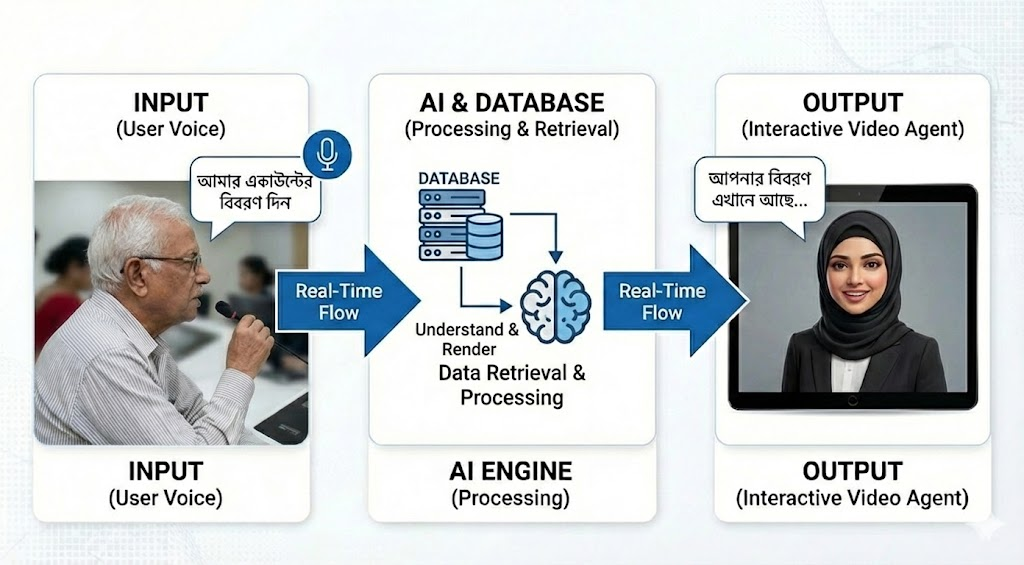
\includegraphics[width=0.8\textwidth]{Graphical_Abstract.jpg}
    \caption{Graphical Abstract}
    \label{fig: Graphical Abstract}
\end{figure}


\section{Project Outcome}

The project delivers a working real-time Bangla conversational avatar. Its main outcomes are:

\begin{itemize}
    \item A complete, running system: browser interface, real-time media layer, Bangla conversational agent and avatar rendering server.
    \item \textbf{Alapon}, a Bangla avatar model built on SyncTalk\_2D, 49~MB in size, rendering at 30 frames per second on a laptop RTX 3050 with 0.3~GB of GPU memory.
    \item Four gaps found and closed in the SyncTalk\_2D model. Covering the jaw stops the mouth moving during silence (41\% of frames $\rightarrow$ 0.1\%).
    \item A Bangla phoneme-to-viseme mapping and a Bangla sound-level evaluation, showing that Alapon's lips close on \bn{প}/\bn{ব}/\bn{ম} and open on \bn{আ}, including for six Bangla speakers it had never heard.
    \item A benchmark of six published systems on Bangla and English video with one scoring code, showing that five of the six leak on at least one dataset and that the standard lip-sync metric scores generated video above real video.
    \item A journal paper in preparation on these findings.
    \item A Bangla audiovisual corpus of 2.78 hours from 24 speakers, used as unseen test audio.
\end{itemize}

\noindent
The system is intended as a foundation for Bangla virtual tutors, public-service assistants, accessible interfaces and interactive media.


\section{Organization of the Report}

\begin{itemize}
    \item \textbf{Chapter 1 - Introduction} presents the problem, motivation, objectives, methodology and outcome of the project.

    \item \textbf{Chapter 2 - Background} covers the concepts needed for the rest of the report, reviews audio-driven talking-head generation and similar applications, and identifies the gap for Bangla.

    \item \textbf{Chapter 3 - Project Design} presents the requirements, the system architecture, how the avatar model was selected and adapted, the gaps found in it, and the project plan.

    \item \textbf{Chapter 4 - Implementation and Results} describes the implementation and reports the effect of closing the model's gaps, Bangla sound-level results, the comparison with published systems, the leakage found in them, and speed and response time.

    \item \textbf{Chapter 5 - Standards and Design Constraints} covers the engineering standards, design constraints, cost, and the complex engineering problem mapping.

    \item \textbf{Chapter 6 - Conclusion} summarises what was delivered against what was proposed, the limitations, the journal paper in progress, and future work.
\end{itemize}

\chapter{Background}
This chapter introduces the concepts used in the rest of the report, reviews the literature on audio-driven talking-head generation and similar applications, and identifies the gap this project addresses.

\section{Preliminaries}
In this section, we provide the background knowledge needed to understand the rest of our report.\\

\noindent
\textbf{Audio-driven talking-head generation:} Generating video of a face whose lip movements follow a given speech signal.

\noindent
\textbf{Person-specific and person-generic models:} A person-specific model is trained for one face and must be retrained for each new person; a person-generic model works on any face without retraining, usually at a higher computational cost.

\noindent
\textbf{U-Net inpainting:} An encoder--decoder network with skip connections. In SyncTalk\_2D it receives a video frame with the mouth region blacked out and ``paints'' the mouth back in, conditioned on the audio.

\noindent
\textbf{Audio features:} Speech is converted into a sequence of numerical features before it reaches the network, for example a mel spectrogram, the output of an audio--visual encoder, or the internal representation of a self-supervised speech model.

\noindent
\textbf{Self-supervised speech encoders (wav2vec~2.0, XLS-R):} Models pre-trained on large amounts of unlabelled speech \cite{baevski2020wav2vec2}. XLS-R \cite{babu2022xlsr} is pre-trained on 128 languages, including Bangla, and its intermediate layers capture phonetic content.

\noindent
\textbf{SyncNet and LSE:} SyncNet \cite{chung2016outoftime} is a network that judges whether a mouth and an audio clip are in sync. From it come the two standard lip-sync metrics: LSE-D (lip-sync error distance; lower is better) and LSE-C (lip-sync error confidence; higher is better).

\noindent
\textbf{Phoneme and viseme:} A phoneme is a distinct speech sound; a viseme is a visually distinct mouth shape. Several phonemes can share a viseme, so a phoneme-to-viseme mapping is many-to-one.

\noindent
\textbf{Leakage:} Mouth motion in a generated video that comes from the input video rather than from the audio. A model that leaks can look well synchronised while ignoring the speech. It is measured by driving the model with silent audio and counting the frames in which the mouth is open \cite{bigata2025keysync}.

\noindent
\textbf{Speech-to-speech conversational model:} A large language model that takes speech in and produces speech out directly, instead of passing through separate speech-recognition and speech-synthesis stages.

\noindent
\textbf{Voice Activity Detection (VAD):} Detecting when a person is speaking, used to decide when the user has finished their turn.

\noindent
\textbf{Real-Time Communication (RTC):} Low-latency streaming of audio and video between browser and server, provided here by LiveKit over WebRTC.

\noindent
\textbf{Neural Radiance Fields (NeRF) and 3D Gaussian Splatting (3DGS):} 3D scene representations used by several recent talking-head systems. NeRF represents the head as a continuous neural field; 3DGS represents it as many small 3D Gaussian ``splats'', which render much faster.


\section{Literature Review}

Speech-driven talking-head synthesis has developed in stages: from 2D image-based animation, to 3D neural representations, to fast Gaussian-Splatting rendering. Each stage addressed the weaknesses of the one before and introduced new trade-offs.\\

\noindent
\textbf{2D animation.} Early work animated a single static image. MakeItTalk \cite{DBLP:journals/corr/abs-2004-12992} separated the speech content from the speaker's identity to drive facial landmarks and head motion from one image, and produced convincing lip-sync and expression control. As a 2D method it did not represent 3D geometry, so head rotation and depth-dependent motion were not consistent.\\

\noindent
\textbf{Neural radiance fields.} To obtain 3D consistency, later work conditioned Neural Radiance Fields on audio. AD-NeRF \cite{DBLP:journals/corr/abs-2103-11078} was the first to do so, producing 3D-consistent, high-fidelity talking faces and upper bodies from new viewpoints. It tied facial motion closely to the radiance field, however, which gave little control over individual facial attributes. DFA-NeRF \cite{DBLP:journals/corr/abs-2201-00791} disentangled lip motion from head pose and blinking for more personalised and controllable generation. NeRF-based methods nonetheless remained slow to train and to render, which made real-time use impractical.\\

\noindent
\textbf{Synchronisation.} SyncTalk \cite{peng2024synctalkdevilsynchronizationtalking} made synchronisation the central problem, aligning audio, lip movement, facial expression and head pose through a face-sync controller and stabilising mechanisms. It clearly improved temporal coherence and realism over earlier NeRF models, but kept NeRF's computational cost.\\

\noindent
\textbf{Gaussian Splatting.} Recent work replaced NeRF with explicit 3D Gaussian Splatting to remove the computational bottleneck. GaussianTalker \cite{cho2024gaussiantalkerrealtimehighfidelitytalking} rendered audio-driven 3D Gaussian talking heads in real time with high visual quality. TalkingGaussian \cite{li2024talkinggaussianstructurepersistent3dtalking} kept the static facial structure separate from the audio-driven deformation, reducing distortion in highly dynamic regions such as the mouth. GaussianSpeech \cite{aneja2024gaussianspeechaudiodrivengaussianavatars} added finer explicit modelling of the teeth and inner mouth, and NeRFFaceSpeech \cite{kim2024nerffacespeechoneshotaudiodriven3d} generated 3D-aware animation from a single image using generative priors. InsTaG \cite{li2025instaglearningpersonalized3d} combined Gaussian Splatting with a universal motion field learned in pre-training, so that a new person can be learned from a few seconds of video.\\

\noindent
\textbf{2D lip-synchronisation.} In parallel, 2D methods edit only the mouth region of an existing video. Wav2Lip \cite{prajwal2020wav2lip} trained a generator against a pre-trained SyncNet ``lip-sync expert'' \cite{chung2016outoftime} and became the most widely used baseline. IP-LAP \cite{zhong2023iplap} adds landmark and appearance priors to preserve identity, and MuseTalk \cite{zhang2024musetalk} and LatentSync \cite{li2024latentsync} generate the mouth in the latent space of an image or diffusion model. SyncTalk\_2D \cite{synctalk2d} is a lightweight person-specific 2D U-Net designed for real-time use, and is the model this project builds on.\\

\noindent
\textbf{Leakage.} Because 2D methods see the rest of the face, they can learn to copy the mouth from the input video instead of generating it from the audio. LatentSync \cite{li2024latentsync} describes this as a shortcut that its training has to counter, and KeySync \cite{bigata2025keysync} proposed a masking strategy against it together with a leakage measure, LipLeak, which drives the model with silent audio. We use the same silent-audio test and extend it in Section~\ref{sec:leakage}.\\

\noindent
\textbf{The gap.} All of these systems are built and tested on high-resource languages, chiefly English, and give little attention to the phonetic and prosodic properties of low-resource languages such as Bangla. The most visually capable methods also need GPUs far beyond consumer hardware, and few report whether the mouth stays still in silence. Our work focuses on a Bangla talking head that runs in real time on a laptop, with its audio dependence verified directly.\\


\subsection{Similar Applications}
\begin{enumerate}
  \renewcommand{\labelenumi}{(\roman{enumi})}

\item
\textbf{Tavus and similar commercial platforms (2024--2025) : }Tavus generates personalised AI-driven talking avatars for sales and marketing, and platforms such as HeyGen offer real-time conversational avatars with voices in many languages, including Bangla. These systems are proprietary, depend on large datasets and cloud-scale compute, are paid per use, and publish no evaluation of how well their lips follow Bangla speech. Our system is open, targets Bangla specifically, measures its Bangla lip movement, and runs its avatar locally on consumer hardware.\\

\begin{figure}[H]
    \centering
    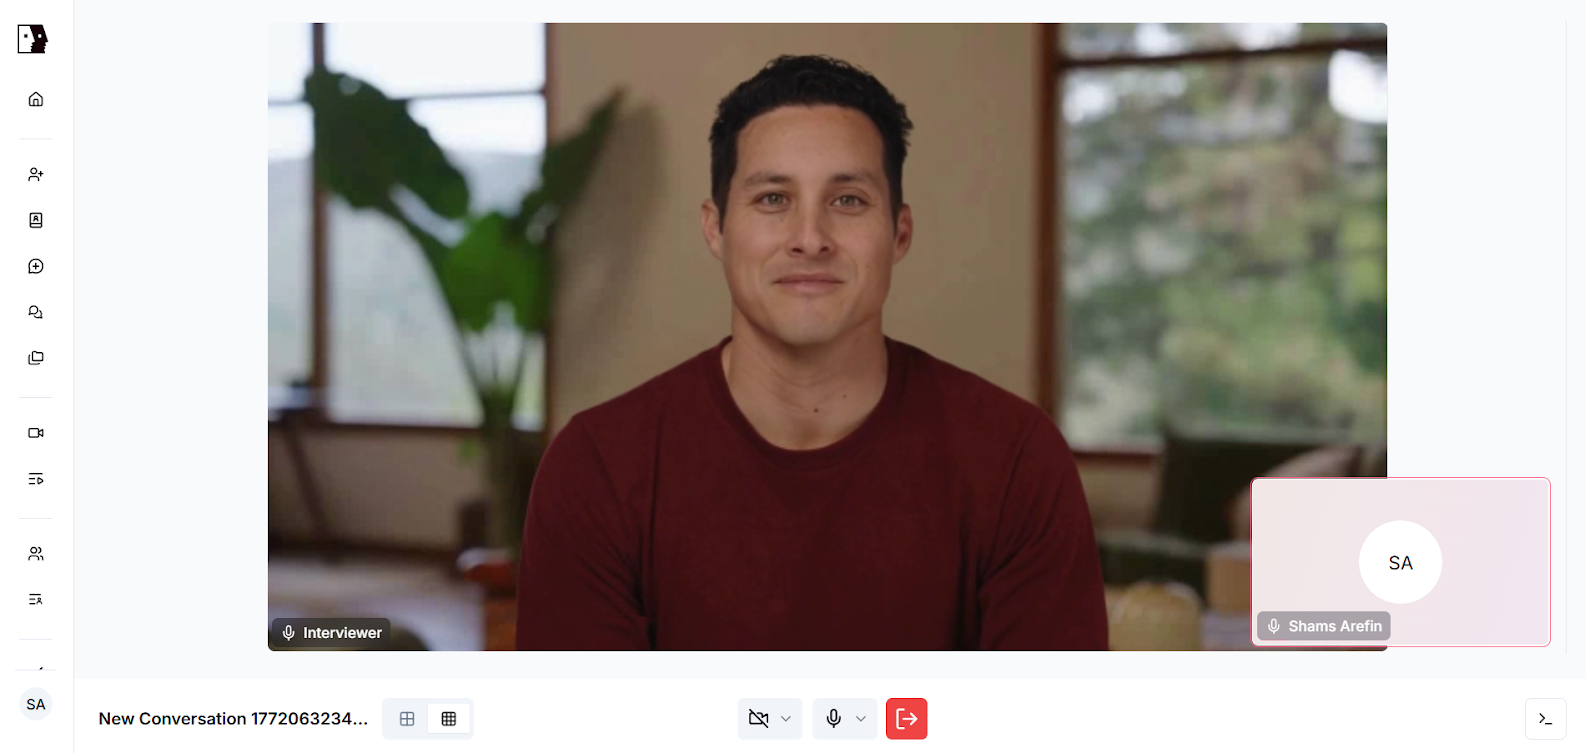
\includegraphics[width=0.8\textwidth]{Tavus.png}
    \caption{Tavus Interface}
    \label{fig: Tavus Interface}
\end{figure}


\item
\textbf{EMO (2024) : }EMO \cite{tian2024emo} generates expressive portrait animation from audio with a 2D diffusion model. It gives very expressive results, but at high computational cost and without real-time operation. Our system trades some expressiveness, since it animates the mouth region only, for real-time rendering on a laptop.\\

\begin{figure}[H]
    \centering
    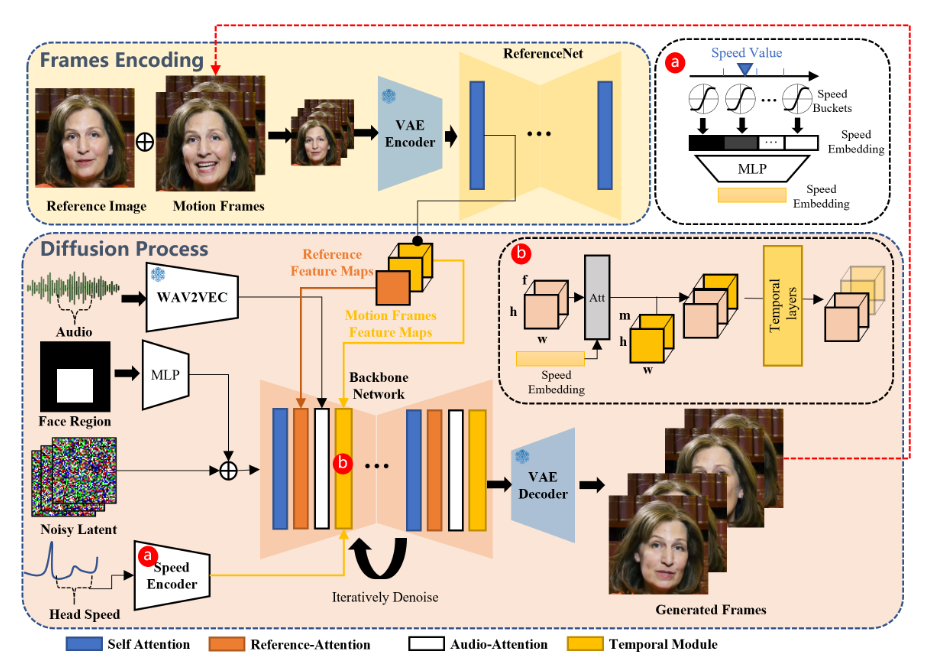
\includegraphics[width=0.8\textwidth]{EMO.png}
    \caption{EMO Methodology}
    \label{fig: EMO Methodology}
\end{figure}


\item
\textbf{SadTalker (2023) : }SadTalker \cite{zhang2023sadtalker} predicts 3D morphable-model parameters from audio and re-renders the face with a neural renderer. It is widely used but suffers from identity drift, unstable eye regions and jittery motion. Because our system edits only the mouth of a real recording of the speaker, the speaker's identity, eyes and head motion come directly from real video.\\

\begin{figure}[H]
    \centering
    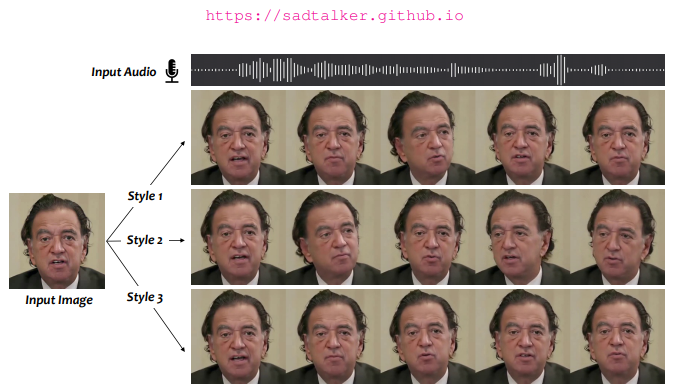
\includegraphics[width=0.8\textwidth]{SadTalker.png}
    \caption{SadTalker}
    \label{fig: SadTalker}
\end{figure}



\item
\textbf{InsTaG (CVPR 2025) : }InsTaG \cite{li2025instaglearningpersonalized3d} is a 3D Gaussian Splatting talking head that combines a universal motion field with a dynamic deformation network, giving strong identity preservation and stable motion. It is trained on English audio. We initially considered InsTaG for this project, but chose a 2D model because our requirement was real-time rendering on a 4~GB laptop GPU.\\

\begin{figure}[H]
    \centering
    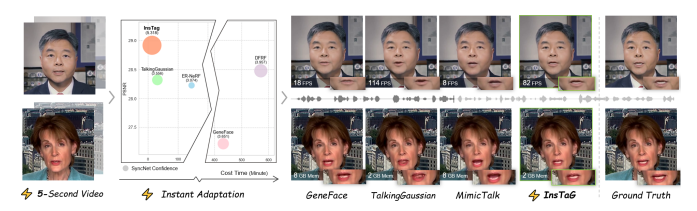
\includegraphics[width=0.8\textwidth]{InsTag.png}
    \caption{InsTaG Methodology}
    \label{fig: InsTag Methodology}
\end{figure}



\item
\textbf{Wav2Lip and SyncNet-based systems : }Wav2Lip \cite{prajwal2020wav2lip} generates the mouth in 2D and is known for strong lip-sync scores. We found that those scores need care: on our Bangla clip and on the public HDTF dataset, Wav2Lip scores \textit{above real video} of the same speaker on the standard lip-sync metric (Section~\ref{sec:leakage}), because it was trained against the same SyncNet that grades it.\\

\begin{figure}[H]
    \centering
    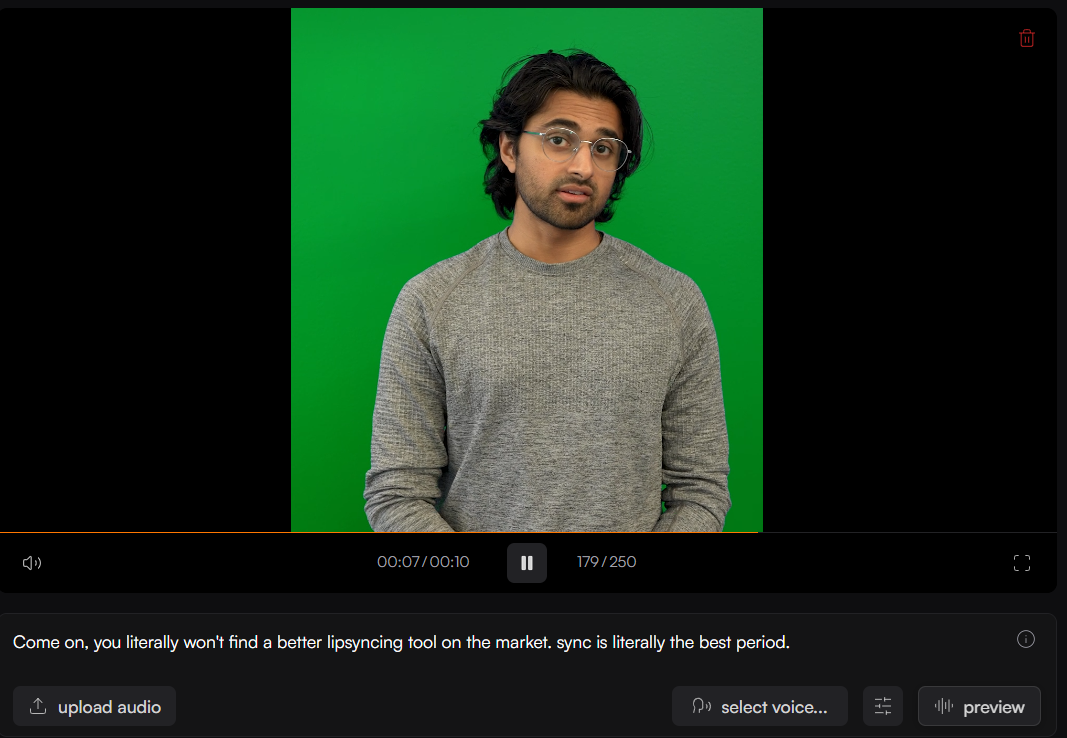
\includegraphics[width=0.8\textwidth]{Wav2Lip.png}
    \caption{Wav2Lip Interface}
    \label{fig: Wav2Lip Interface}
\end{figure}



\item
\textbf{NeRF-based head avatars : }Models such as AD-NeRF \cite{DBLP:journals/corr/abs-2103-11078} give high-quality reenactment but need long training and struggle with head poses outside the training data. Gaussian Splatting models render faster, but still need more GPU than a consumer laptop provides.\\

\end{enumerate}



\section{Gap Analysis}

\begin{table}[H]
\centering
\caption{Comparison of existing talking-head synthesis methods with the proposed system}
\label{tab:comparison}
\renewcommand{\arraystretch}{1.3}

\adjustbox{max width=\textwidth}{
\begin{tabular}{|p{4.2cm}|c|c|c|c|c|c|}
\hline
\textbf{Paper}
& \textbf{SyncTalk}
& \textbf{GaussianTalker}
& \textbf{InsTaG}
& \textbf{TalkingGaussian}
& \textbf{NeRFFaceSpeech}
& \textbf{Alapon (ours)} \\
\hline

Speech-driven talking head generation
& \cmark & \cmark & \cmark & \cmark & \cmark & \cmark \\
\hline

Trained and evaluated on Bangla speech
& \xmark & \xmark & \xmark & \xmark & \xmark & \cmark \\
\hline

Bangla-trained lip-sync expert
& \xmark & \xmark & \xmark & \xmark & \xmark & \cmark \\
\hline

Bangla audio-visual dataset
& \xmark & \xmark & \xmark & \xmark & \xmark & \cmark \\
\hline

Real-time shown on a laptop GPU$^{*}$
& \xmark & \xmark & \xmark & \xmark & \xmark & \cmark \\
\hline

Silent-audio leakage test reported$^{*}$
& \xmark & \xmark & \xmark & \xmark & \xmark & \cmark \\
\hline

Phoneme-level (viseme) supervision
& \xmark & \xmark & \xmark & \xmark & \xmark & partial$^{\dagger}$ \\
\hline

\end{tabular}
}

\vspace{0.3em}
{\footnotesize $^{*}$As reported in the original publications, which evaluate on desktop or datacentre GPUs. $^{\dagger}$A Bangla phoneme-to-viseme mapping is defined and used for evaluation; using it as a training signal is future work.}
\end{table}

\noindent
Current talking-head systems achieve speech-driven animation with high visual quality, but none of those in Table~\ref{tab:comparison} is trained or evaluated on Bangla, and none reports whether its mouth stays still when the audio is silent, the simplest test that the mouth is actually driven by the audio. Most also require GPUs well beyond consumer hardware. The proposed system addresses these gaps with Bangla training data, a Bangla-trained lip-sync expert, a silent-audio leakage test, and a model small enough to run in real time on a laptop. Phoneme-level lip-shape supervision is only partly addressed and is identified as future work.

\section{Summary}
Current talking-head systems such as SyncTalk, InsTaG, GaussianTalker and NeRFFaceSpeech have made major advances in high-quality audio-driven facial synthesis using NeRF and 3D Gaussian Splatting, reaching impressive realism and, in some cases, real-time rendering on powerful GPUs. 2D lip-synchronisation methods such as Wav2Lip, MuseTalk and LatentSync are widely used for dubbing. Almost all of them, however, are developed and evaluated on high-resource languages, and rarely check whether their mouth motion is truly driven by the audio. This motivates a real-time Bangla speech-driven avatar that is trained on Bangla data, verified to be driven by the audio rather than by the input video, and light enough to run on consumer hardware.\\

\chapter{Project Design}

This chapter presents the requirements of the system, its architecture, how the avatar model was selected, adapted to Bangla and improved, and the project plan.

\section{Requirement Analysis}
The system has two very different computational profiles. \textit{Training} the avatar model is done once per avatar and needs a datacentre-class GPU; we used Google Colab (NVIDIA A100 and L4). \textit{Running} the system must fit on consumer hardware: the avatar renderer runs locally on a laptop NVIDIA RTX 3050 with 4~GB of memory, while conversational reasoning is handled by a cloud API. The project also requires Bangla audiovisual data for training and evaluation, and enough local storage for video frames, landmarks and audio features.


\subsection{Functional and Nonfunctional Requirements}

\subsubsection{Functional Requirements}

\begin{enumerate}
    \item \textbf{Interface:} The system captures the user's microphone audio in a web browser and displays the avatar's video and audio reply, with a live transcript.

    \item \textbf{Secured Real-Time Communication Layer (RTC):} Audio and video are streamed between the user and the system over LiveKit, with access tokens issued by a token server.

    \item \textbf{Conversational Processing Module:} The agent detects the end of the user's turn, understands the Bangla request, and generates a spoken Bangla reply that keeps the conversation history.

    \item \textbf{Speech Output:} The reply is produced directly as Bangla speech by the speech-to-speech conversational model.

    \item \textbf{Talking-Head Video Generation \& Streaming:} The avatar server turns the reply audio into lip-synchronised video frames, streams them in step with the audio, and plays an idle animation when the avatar is not speaking.
\end{enumerate}


\subsubsection{Non-Functional Requirements}

\begin{enumerate}
    \item \textbf{Availability:} The system is accessible whenever the server is running, with minimal downtime.

    \item \textbf{Security:} Users are authenticated through session tokens.

    \item \textbf{Performance \& Quality:} The system answers within 1--2 seconds of the user finishing speaking, and the avatar renders at no less than 25 frames per second.

    \item \textbf{Reliability:} The system runs on a consumer laptop GPU without exhausting its memory.

    \item \textbf{Linguistic Robustness:} Bangla speech is transcribed in Bangla script and answered in natural, formal-register Bangla.

    \item \textbf{Modularity \& Scalability:} The conversational agent, the real-time media layer and the avatar renderer are decoupled, so each can be upgraded or replaced independently.
\end{enumerate}


\subsection{System Diagram}
The system diagram is depicted in Figure~\ref{fig:SystemDiagram}, which gives a high-level overview of our system.
\begin{figure}[H]
    \centering
    \begin{tikzpicture}[
        node distance=0.9cm and 1.2cm,
        box/.style={draw=axisgrey, fill=restsoft, rounded corners, align=center, minimum width=4.6cm, minimum height=1.05cm, font=\small, text=inkc},
        local/.style={box},
        cloud/.style={box, dashed},
        alapon/.style={box, draw=alaponblue, fill=alaponsoft, line width=0.9pt, text=alapondark},
        arr/.style={{Stealth[length=2mm]}-{Stealth[length=2mm]}, thick, draw=inkc},
        barr/.style={arr, draw=alaponblue},
        lbl/.style={font=\footnotesize, fill=white, inner sep=1.5pt, text=inkgrey}]
      \node[box, fill=white] (user) {User};
      \node[local, below=of user] (browser) {Browser client\\ microphone, avatar video, transcript};
      \node[local, right=of browser, minimum width=3.4cm] (token) {Token server\\ (Flask)};
      \node[cloud, below=of browser] (lk) {LiveKit Cloud\\ real-time audio and video};
      \node[local, below=of lk] (agent) {Bangla agent\\ LiveKit Agents, Silero VAD};
      \node[cloud, right=of agent, minimum width=3.4cm] (gemini) {Gemini 3.1 Flash Live\\ (cloud API)};
      \node[alapon, below=of agent] (avatar) {Avatar server\\ \textbf{Alapon} on the laptop GPU};
      \draw[arr] (user) -- node[lbl, right] {speech / avatar} (browser);
      \draw[arr] (browser) -- node[lbl, above] {token} (token);
      \draw[arr] (browser) -- node[lbl, right] {audio / video} (lk);
      \draw[arr] (lk) -- node[lbl, right] {audio / video} (agent);
      \draw[arr] (agent) -- node[lbl, above] {speech} (gemini);
      \draw[barr] (agent) -- node[lbl, right, text=alapondark] {reply audio / frames} (avatar);
    \end{tikzpicture}

    \vspace{0.3em}
    {\footnotesize\color{inkgrey} Dashed border: cloud service. Blue: Alapon, the avatar model, running on the laptop.}
    \caption{System Diagram}
    \label{fig:SystemDiagram}
\end{figure}

\subsection{Sequence Diagram}
The sequence diagram is depicted in Figure~\ref{fig:SequenceDiagram}, which shows the order of interactions between the components during one conversational turn.
\begin{figure}[H]
    \centering
    \resizebox{\textwidth}{!}{%
    \begin{tikzpicture}[
        head/.style={draw=axisgrey, rounded corners, fill=restsoft, align=center, minimum width=2.1cm, minimum height=0.9cm, font=\small, text=inkc},
        ahead/.style={head, draw=alaponblue, fill=alaponsoft, text=alapondark, line width=0.9pt},
        msg/.style={-{Stealth[length=2mm]}, thick, draw=inkc},
        ret/.style={msg, dashed},
        bmsg/.style={msg, draw=alaponblue},
        bret/.style={bmsg, dashed},
        lbl/.style={font=\footnotesize, above, inner sep=1.5pt, align=center, text=inkgrey},
        note/.style={draw=axisgrey, fill=restsoft, font=\footnotesize, align=center, inner sep=2pt, text=inkc},
        anote/.style={note, draw=alaponblue, fill=alaponsoft, text=alapondark}]
      \foreach \x/\name/\txt in {0/U/User, 2.6/B/Browser\\client, 5.2/T/Token\\server, 7.8/L/LiveKit, 10.4/A/Bangla\\agent, 13.0/G/Gemini\\Live}{
        \node[head] (\name) at (\x,0) {\txt};
        \draw[restgrey, thick] (\x,-0.45) -- (\x,-12.6);
      }
      \node[ahead] (V) at (15.6,0) {Avatar server\\ (Alapon)};
      \draw[alaponblue!45, thick] (15.6,-0.45) -- (15.6,-12.6);
      \draw[msg] (2.6,-1.1) -- node[lbl] {request token} (5.2,-1.1);
      \draw[ret] (5.2,-1.8) -- node[lbl] {token} (2.6,-1.8);
      \draw[msg] (2.6,-2.5) -- node[lbl] {join room} (7.8,-2.5);
      \draw[msg] (0,-3.2) -- node[lbl] {speaks Bangla} (2.6,-3.2);
      \draw[msg] (2.6,-3.9) -- node[lbl] {microphone audio} (7.8,-3.9);
      \draw[msg] (7.8,-4.6) -- node[lbl] {user audio} (10.4,-4.6);
      \node[note] at (10.4,-5.4) {VAD: end of turn\\ after 0.55 s of silence};
      \draw[msg] (10.4,-6.3) -- node[lbl] {user speech} (13.0,-6.3);
      \draw[ret] (13.0,-7.0) -- node[lbl] {reply speech + transcript} (10.4,-7.0);
      \draw[bmsg] (10.4,-7.7) -- node[lbl, text=alapondark] {reply audio (24 kHz PCM)} (15.6,-7.7);
      \node[anote] at (15.6,-8.5) {Alapon renders\\ lip-synced frames};
      \draw[bret] (15.6,-9.4) -- node[lbl, text=alapondark] {frames + audio segments} (10.4,-9.4);
      \draw[msg] (10.4,-10.1) -- node[lbl] {publish audio + video} (7.8,-10.1);
      \draw[msg] (7.8,-10.8) -- node[lbl] {audio + video} (2.6,-10.8);
      \draw[msg] (2.6,-11.5) -- node[lbl] {avatar speaks} (0,-11.5);
      \node[note, minimum width=13.6cm] at (8.9,-12.2) {Idle animation is streamed whenever the avatar is not speaking};
    \end{tikzpicture}}
    \caption{Sequence Diagram of the Proposed System}
    \label{fig:SequenceDiagram}
\end{figure}




\subsection{UI Design}

\begin{figure}[H]
    \centering
    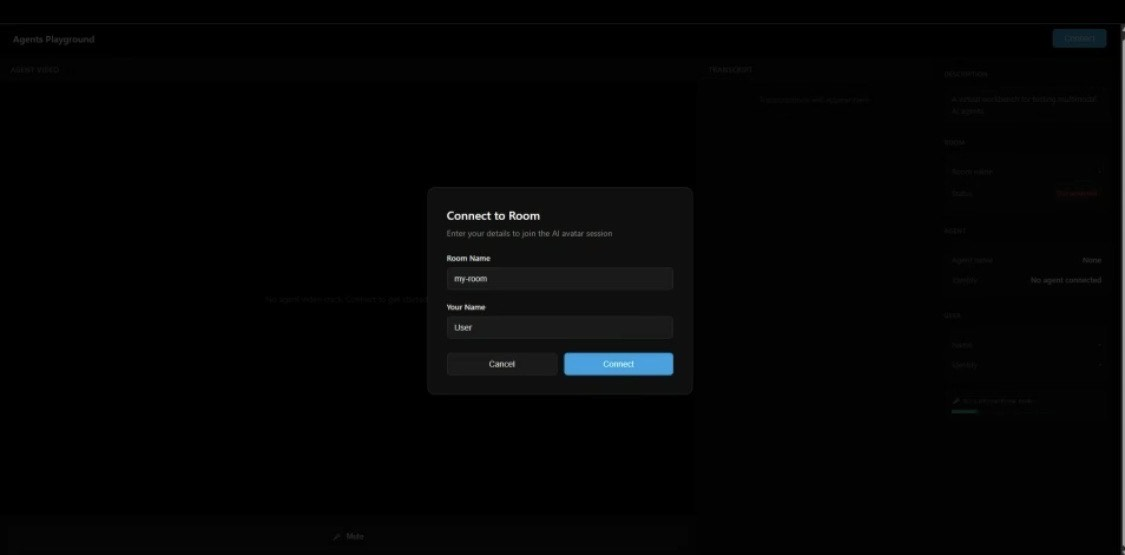
\includegraphics[width=0.8\textwidth]{UI1.jpeg}
    \caption{User Interface of our System}
    \label{fig: User Interface of our System}
\end{figure}


\begin{figure}[H]
    \centering
    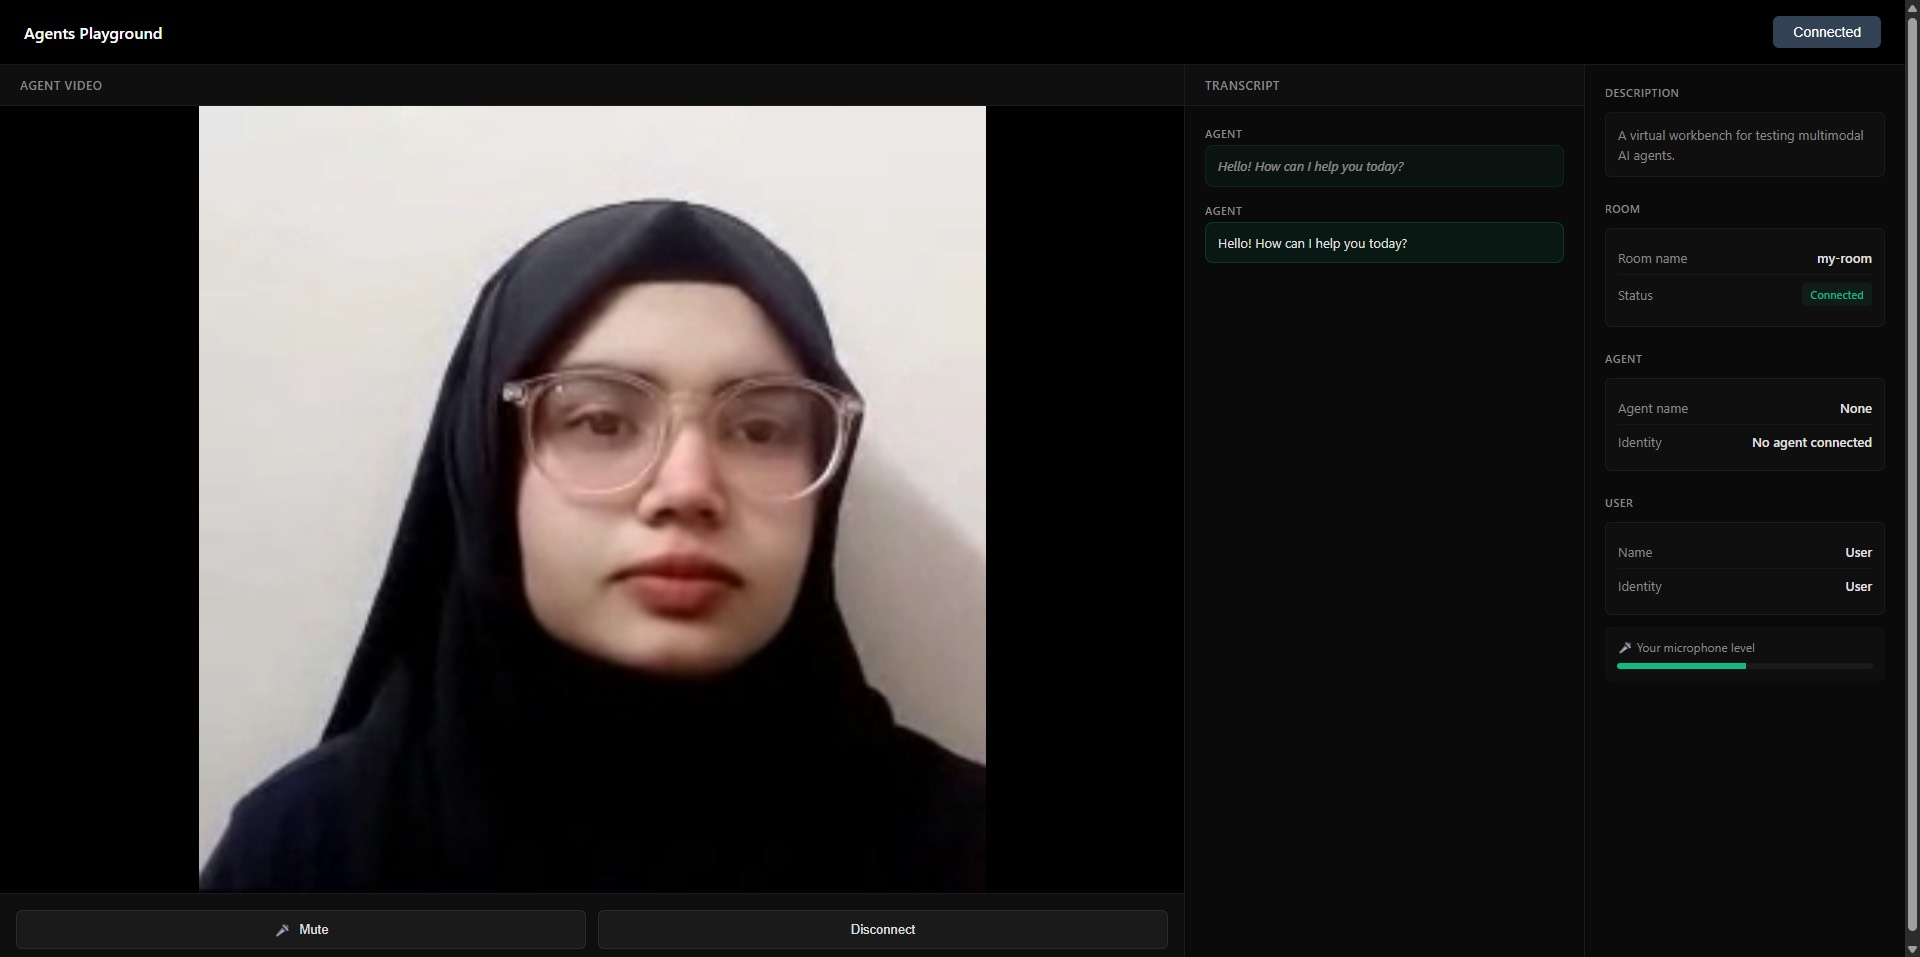
\includegraphics[width=0.8\textwidth]{UI2.jpeg}
    \caption{User Interface of our System}
    \label{fig: User Interface of our System 2}
\end{figure}


\section{Detailed Methodology and Design}

This section describes the architecture of the delivered system, how the design evolved, the Bangla conversational agent, the avatar rendering server, and how the avatar model was selected, adapted to Bangla and improved.

\subsubsection{Overall System Architecture}

The system is a voice-to-voice-and-video pipeline:

\begin{center}
\textit{Speech $\rightarrow$ Conversational model $\rightarrow$ Speech $\rightarrow$ Audio features $\rightarrow$ Lip-synchronised video}
\end{center}

\noindent
The user speaks Bangla in the browser. The audio reaches the agent over LiveKit. The agent's conversational model produces a spoken Bangla reply, which is sent to the avatar server. The avatar server converts the reply audio into lip-synchronised video frames and streams them back, and the agent publishes the audio and video together to the user through LiveKit. The components are independent processes connected by LiveKit and WebSockets, so each can be developed, debugged and replaced separately.


\begin{figure}[H]
    \centering
    \resizebox{\textwidth}{!}{%
    \begin{tikzpicture}[
        comp/.style={draw=axisgrey, rounded corners, fill=white, align=center, font=\small, minimum height=0.95cm, minimum width=3.3cm, text=inkc},
        acomp/.style={comp, draw=alaponblue, fill=alaponsoft, text=alapondark, line width=0.9pt},
        layer/.style={draw=axisgrey, dashed, rounded corners, inner sep=8pt, fill=restsoft},
        ttl/.style={font=\small\bfseries, anchor=south west, inner sep=2pt, text=inkc},
        arr/.style={-{Stealth[length=2mm]}, thick, draw=inkc},
        barr/.style={arr, draw=alaponblue},
        lbl/.style={font=\footnotesize, fill=white, inner sep=1.5pt, align=center, text=inkgrey}]
      % client layer
      \node[comp] (browser) at (0,0) {Browser client\\ mic, video, transcript};
      \node[comp] (token) at (4.2,0) {Token server\\ (Flask)};
      % rtc
      \node[comp, dashed, minimum width=7.5cm] (lk) at (2.1,-2.1) {LiveKit Cloud (WebRTC): real-time audio and video};
      % agent
      \node[comp] (vad) at (0,-4.4) {Silero VAD\\ end of turn: 0.55 s};
      \node[comp] (sess) at (4.2,-4.4) {Gemini session\\ bn-BD, persona, phrases};
      \node[comp, dashed] (gem) at (9.4,-4.4) {Gemini 3.1 Flash Live\\ speech-to-speech (cloud)};
      % avatar
      \node[comp] (feat) at (0,-7.0) {Streaming audio\\ features};
      \node[acomp] (unet) at (4.2,-7.0) {\textbf{Alapon}\\ U-Net renderer};
      \node[comp] (jpeg) at (8.4,-7.0) {JPEG frames +\\ segment protocol};
      \node[comp] (idle) at (8.4,-8.6) {Idle frame cache};
      \begin{scope}[on background layer]
        \node[layer, fit=(browser)(token)] (L1) {};
        \node[layer, fit=(lk)] (L2) {};
        \node[layer, fit=(vad)(sess)] (L3) {};
        \node[layer, fill=alaponsoft!45, draw=alaponblue!60, fit=(feat)(unet)(jpeg)(idle)] (L4) {};
      \end{scope}
      \node[ttl] at (L1.north west) {Client layer};
      \node[ttl] at (L2.north west) {Real-time communication layer};
      \node[ttl] at (L3.north west) {Bangla agent (LiveKit Agents)};
      \node[ttl, text=alapondark] at (L4.north west) {Avatar server (FastAPI, laptop GPU)};
      \draw[arr] (token) -- (browser);
      \draw[arr, {Stealth[length=2mm]}-{Stealth[length=2mm]}] (browser) -- (browser |- lk.north);
      \draw[arr, {Stealth[length=2mm]}-{Stealth[length=2mm]}] (vad |- lk.south) -- (vad);
      \draw[arr] (vad) -- node[lbl, above] {turn} (sess);
      \draw[arr, {Stealth[length=2mm]}-{Stealth[length=2mm]}] (sess) -- node[lbl, above] {speech} (gem);
      \draw[barr] (sess) -- node[lbl, right, text=alapondark] {reply audio\\ 24 kHz PCM} (sess |- L4.north);
      \draw[barr] (feat) -- (unet);
      \draw[barr] (unet) -- (jpeg);
      \draw[barr] (jpeg.north) -- ++(0,1.2) -| node[lbl, pos=0.25, text=alapondark] {frames + audio} (sess.south east);
      \draw[arr] (idle) -- (jpeg);
    \end{tikzpicture}}
    \caption{System Architecture}
    \label{fig:SystemArchitecture}
\end{figure}

\noindent
\textbf{How the design evolved.} The FYDP-1 design was a cascade of three separate services: Whisper speech recognition through a Gradio API, Gemini 2.5 Flash for text reasoning, and Microsoft Edge TTS (\texttt{bn-IN-TanishaaNeural}) for speech synthesis. Each stage added its own latency, so we moved to Gemini's speech-to-speech ``native audio'' model, which removed the separate recognition and synthesis stages. That model, however, slowed down as a conversation went on: its reply time grew from 8 seconds to 66 seconds within five turns. Switching to \texttt{gemini-3.1-flash-live-preview} kept the reply time constant, and this is the model used in the final system.

\vspace{0.5em}

\subsubsection{Real-Time Communication Layer and Agent Control}

The agent is built on the LiveKit Agents framework \cite{livekitagents}. It creates the LiveKit session, greets the user, and then listens continuously, routing the user's audio to the conversational model and the reply to the avatar server. It manages the session lifecycle and user interruptions, so the interaction behaves like a conversation rather than a request--response exchange. A small Flask server issues the LiveKit access tokens used by the browser.

\vspace{0.5em}

\subsubsection{Bangla Conversational Agent}

The conversational model \cite{geminilive} receives the user's speech directly and replies in speech. Three Bangla-specific problems appeared that do not occur in English, and each needed its own fix.

\begin{itemize}
    \item \textbf{Wrong script in the transcript.} By default the model detected the language afresh on every utterance. With short turns of 0.6--1.8 seconds, phonetic overlap between Bangla, Hindi and Punjabi, and English loanwords, the same speaker's words came back in Devanagari, Gurmukhi and Roman script within a single session. We pinned the input language to \texttt{bn-BD}.
    \item \textbf{Turns cut off mid-question.} Bangla speakers pause mid-sentence, and the default end-of-turn detection answered half a question. We run a local voice-activity detector (Silero \cite{silero2021}) with the end-of-turn silence set to 0.55 seconds, long enough to survive a natural Bangla pause.
    \item \textbf{Technical vocabulary pulled towards English.} Terms such as ``\bn{মেশিন লার্নিং}'' and ``ChatGPT'' repeatedly shifted recognition away from Bangla. We supply them as biasing phrases.
\end{itemize}

\noindent
The agent's persona, ``Redwan'', answers only in Bangla, in the formal register (\bn{আপনি}), and keeps established technical terms in their usual form.

\vspace{0.5em}

\subsubsection{Avatar Rendering Server}

The avatar server is a FastAPI application with WebSocket endpoints for audio in and video out. At 25 frames per second it has a budget of 40~ms per frame.

\begin{itemize}
    \item \textbf{Streaming audio features.} The model was trained on audio features extracted from whole recordings, but live audio arrives in chunks. Extracting features chunk by chunk shifts the timeline slightly at every boundary and slowly desynchronises the lips. Our streaming feature extractor produces the same features as offline extraction: it resamples with a fixed phase, recomputes mel frames from a hop-aligned tail with eight frames of context, and emits a feature only once all of its audio has arrived.
    \item \textbf{Segment protocol.} Each reply segment carries its frame count and its audio, so the client knows exactly how many frames to expect and plays them against the audio.
    \item \textbf{Audio never waits for video.} If a frame is late the previous frame is repeated, because a gap in the voice is far more noticeable than a repeated frame.
    \item \textbf{Cached source frames and idle animation.} Decoded video frames and their landmarks are cached in memory, and idle frames are pre-rendered, so the GPU is free to render speech when it arrives.
\end{itemize}

\vspace{0.5em}

\subsubsection{Selecting the Avatar Model}
\label{sec:selection}

The avatar model must render at least 25 frames per second on a 4~GB laptop GPU while the rest of the system is running, and its lips must follow Bangla speech. We chose SyncTalk\_2D for its size and speed, and confirmed the choice by running the published lip-sync systems that have public code and weights on the same 31-second Bangla clip (Table~\ref{tab:candidates}). Their lip-sync results are in Section~\ref{sec:comparison}.

\begin{table}[H]
\centering
\caption{Candidate avatar models against the project requirements}
\label{tab:candidates}
\renewcommand{\arraystretch}{1.3}
\begin{tabular}{|p{3.1cm}|p{4.4cm}|r|p{3.2cm}|}
\hline
\textbf{Model} & \textbf{Type} & \textbf{Checkpoint file} & \textbf{Time for the 31 s clip (T4)$^{*}$} \\
\hline
\textbf{SyncTalk\_2D} \cite{synctalk2d} & 2D, person-specific & \textbf{49 MB} & \textbf{2 min 33 s} \\
\hline
Wav2Lip \cite{prajwal2020wav2lip} & 2D, person-generic & 436 MB$^{\dagger}$ & 9 min 06 s \\
\hline
IP-LAP \cite{zhong2023iplap} & 2D, person-generic & 475 MB & not timed \\
\hline
MuseTalk 1.5 \cite{zhang2024musetalk} & 2D latent, person-generic & 3,400 MB & about 15 min \\
\hline
LatentSync 1.5 \cite{li2024latentsync} & 2D latent diffusion, person-generic & 5,072 MB & about 30 min \\
\hline
InsTaG \cite{li2025instaglearningpersonalized3d} & 3D Gaussian Splatting, person-specific & -- & not run \\
\hline
\end{tabular}

\vspace{0.3em}
{\footnotesize $^{*}$Offline generation on a cloud T4 GPU, including each system's one-off preprocessing and video file reading and writing; this is not a measure of live speed. $^{\dagger}$Wav2Lip's file also stores training optimiser state, so its model weights are smaller than the file. IP-LAP: its two checkpoints together.}
\end{table}

\begin{figure}[H]
    \centering
    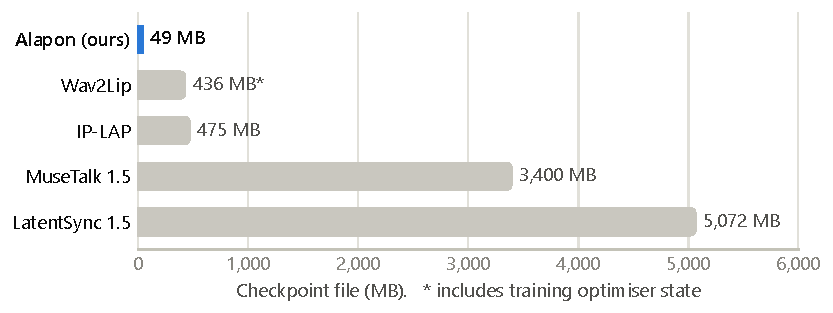
\includegraphics[width=\textwidth]{fig_model_size.pdf}
    \caption{Checkpoint size of the candidate models}
    \label{fig:modelsize}
\end{figure}

\noindent
SyncTalk\_2D has the smallest model and generated the clip fastest. LatentSync's model file alone is larger than the laptop's 4~GB of GPU memory, and MuseTalk's nearly fills it. InsTaG was ruled out because 3D Gaussian Splatting training and rendering exceed the 4~GB laptop budget. The person-generic systems can animate any face without training; SyncTalk\_2D's cost is that it must be trained for each face (about five minutes of video and seven hours of training), which is acceptable for an avatar that represents one fixed speaker. Being person-specific also means the speaker's identity, eyes and head motion come directly from real video; only the mouth is generated.

\vspace{0.5em}

\subsubsection{Alapon: Adapting SyncTalk\_2D to Bangla}

SyncTalk\_2D \cite{synctalk2d} is a 2D U-Net that receives two images, a reference frame of the speaker and the current frame with the mouth region blacked out, together with audio features, and paints the mouth back in (Figure~\ref{fig:Alapon}). \textbf{Alapon} is SyncTalk\_2D adapted to Bangla and improved in the following ways.

\begin{figure}[H]
    \centering
    \resizebox{0.95\textwidth}{!}{%
    \begin{tikzpicture}[
        blk/.style={draw=axisgrey, fill=restsoft, rounded corners, align=center, font=\small, minimum height=1cm, minimum width=3.2cm, text=inkc},
        arr/.style={-{Stealth[length=2mm]}, thick, draw=inkc},
        lbl/.style={font=\footnotesize, fill=white, inner sep=1.5pt, align=center, text=inkgrey}]
      % inputs
      \node[blk] (ref) at (0,2.2) {Reference frame\\ (one fixed frame)};
      \node[blk] (msk) at (0,0.6) {Current frame,\\ mouth and jaw hidden};
      \node[blk] (aud) at (0,-1.0) {Audio features\\ (streamed live)};
      \node[blk, draw=alaponblue, fill=alaponsoft, text=alapondark, line width=0.9pt, minimum height=3.8cm] (unet) at (4.6,0.6) {\textbf{Alapon}\\ U-Net};
      \node[blk, fill=white] (out) at (8.8,0.6) {Generated mouth\\ pasted into frame};
      \node[blk, dashed, fill=white] (sync) at (4.6,-2.4) {Bangla lip-sync expert\\ (training only)};
      \draw[arr] (ref) -- (unet.west |- ref);
      \draw[arr] (msk) -- (unet);
      \draw[arr, draw=alaponblue] (aud) -- (unet.west |- aud);
      \draw[arr, draw=alaponblue] (unet) -- (out);
      \draw[arr, dashed, draw=axisgrey] (out.south) |- node[lbl, pos=0.75] {sync loss} (sync.east);
      % mask inset: orange = the jaw the original mask left visible
      \begin{scope}[shift={(11.6,-0.9)}]
        \node[font=\footnotesize\bfseries, text=leakorange] at (0.7,3.5) {Original mask};
        \draw[axisgrey, fill=white] (0,0) rectangle (1.4,3.2);
        \fill[inkc] (0.15,0.25) rectangle (1.25,1.7);
        \fill[leaksoft] (0.15,0) rectangle (1.25,0.25);
        \draw[leakorange, thick] (0.15,0) rectangle (1.25,0.25);
        \node[font=\scriptsize, text=leakorange, align=center] at (0.7,-0.28) {jaw visible};
        \node[font=\footnotesize\bfseries, text=alapondark] at (2.6,3.5) {Alapon};
        \draw[axisgrey, fill=white] (1.9,0) rectangle (3.3,3.2);
        \fill[inkc] (2.05,0) rectangle (3.15,1.7);
        \node[font=\scriptsize, text=white] at (2.6,0.9) {hidden};
        \node[font=\scriptsize, text=alapondark, align=center] at (2.6,-0.28) {jaw hidden};
      \end{scope}
    \end{tikzpicture}}
    \caption{Alapon: inputs, output and the change to the mouth mask}
    \label{fig:Alapon}
\end{figure}

\noindent
\textbf{1. Bangla training data.} The avatar is trained on 7,717 frames (about 5.1 minutes) of a Bangla speaker, \texttt{redwan}, at 25~fps and 1080$\times$1080. The recording is split into contiguous intervals: frames 0--6170 for training, 6171--6941 for validation, and 6942--7713 (772 frames) for testing. Contiguous intervals are used because neighbouring frames are almost identical, and a random split would put near-copies of test frames into training.\\

\noindent
\textbf{2. Bangla lip-sync expert.} During training, a SyncNet ``expert'' judges whether the generated mouth matches the audio. We retrained the expert on the Bangla speaker with contrastive sampling: half of all training pairs are mismatched, so the expert must learn to tell a correct mouth from a shifted one. The avatar was trained against this Bangla expert, with the sync loss switched on from epoch 5 at a weight of 0.03.\\

\noindent
\textbf{3. Streaming audio features} for the live system, described above.\\

\noindent
\textbf{4. Multilingual audio encoder (XLS-R).} The default audio features come from an audio--visual encoder trained on English. We also tried XLS-R \cite{babu2022xlsr}, a speech encoder pre-trained on 128 languages including Bangla, in place of these features. It did not work (Section~\ref{sec:xlsr}), so Alapon uses the default features.\\

\noindent
\textbf{5. Closing the model's performance gaps.} While training the Bangla model we found that its mouth moved even when the audio was silent, and its lips did not close fully on \bn{প}, \bn{ব}, \bn{ম}. Investigating this revealed four gaps in the SyncTalk\_2D model that held back its performance (Table~\ref{tab:gaps}). Alapon addresses all four. Only the first is measured directly on its own (Section~\ref{sec:maskfix}); the other three are design and training issues that we corrected together.

\begin{table}[H]
\centering
\caption{Gaps in the SyncTalk\_2D model and how Alapon addresses them}
\label{tab:gaps}
\renewcommand{\arraystretch}{1.3}
\begin{tabular}{|p{4.2cm}|p{5.3cm}|p{3.7cm}|}
\hline
\textbf{Gap in the model} & \textbf{Effect on performance} & \textbf{How Alapon addresses it} \\
\hline
\textbf{The mouth mask does not cover the jaw.} The mouth region should be fully hidden, but the bottom ten rows of the face crop (the chin and jaw) stay visible in training and in use. & The model reads mouth opening from the visible jaw instead of the audio, so the mouth moves during silence and lip closures are weak. With audio and reference held constant, this ten-pixel strip produced \textbf{91\% of all mouth motion}. & Mask extended to cover the jaw (Section~\ref{sec:maskfix}). \\
\hline
\textbf{The lip-sync expert learns only from matching audio--video pairs.} & It never sees an out-of-sync example, so it approves every mouth and gives no useful training signal, consistent with the FYDP-1 observation that SyncNet scores stayed near 1.0 at every offset. & Expert retrained with mismatched pairs (item 2). \\
\hline
\textbf{The lip-sync loss is weighted 10$\times$.} & Together with the gap above, a strong training signal that carries no real information about synchronisation. & Weight 0.03, switched on from epoch 5. \\
\hline
\textbf{Training and use see different reference frames.} & A mismatch between what the model learns and what it sees at run time. & One fixed reference frame in both. A control run showed this changes leakage by only 1\%. \\
\hline
\end{tabular}
\end{table}

\noindent
\textbf{6. A clean training split.} While preparing the final training runs we also found that training had drawn frames, including reference frames, from the whole video, test interval included. Training now uses only the training interval, and the interval is recorded with each trained model. The models evaluated in this report were trained before this change; Section~\ref{sec:testing} explains which results this affects.\\

\noindent
\textbf{7. Bangla phoneme-to-viseme mapping.} A \textit{viseme} is a visually distinct mouth shape; several phonemes can share one. Table~\ref{tab:viseme} maps the Bangla sound inventory to eleven visemes.

\begin{table}[H]
\centering
\caption{Bangla phoneme-to-viseme mapping}
\label{tab:viseme}
\renewcommand{\arraystretch}{1.3}
\begin{tabular}{|p{1.1cm}|p{4.2cm}|p{4.3cm}|p{3.6cm}|}
\hline
\textbf{Viseme} & \textbf{Mouth shape} & \textbf{Bangla letters} & \textbf{Phonemes (IPA)} \\
\hline
V0 & Rest, lips closed & (silence, pause) & -- \\
\hline
V1 & Lips pressed together & \bn{প ফ ব ভ ম} & {\ipafont /p pʰ b bʱ m/} \\
\hline
V2 & Lips apart, neutral; tongue at teeth or ridge & \bn{ত থ দ ধ ট ঠ ড ঢ ড় ঢ় ন ণ ল র স ৎ} & {\ipafont /t̪ t̪ʰ d̪ d̪ʱ ʈ ʈʰ ɖ ɖʱ ɽ ɽʱ n l r s/} \\
\hline
V3 & Lips slightly protruded & \bn{চ ছ জ ঝ য শ ষ} & {\ipafont /tʃ tʃʰ dʒ dʒʱ ʃ/} \\
\hline
V4 & Neutral; jaw follows the vowel & \bn{ক খ গ ঘ ঙ ং হ} & {\ipafont /k kʰ g gʱ ŋ ɦ/} \\
\hline
V5 & Spread, close & \bn{ই ঈ} & {\ipafont /i/} \\
\hline
V6 & Spread, mid-open & \bn{এ}, \bn{অ্যা} & {\ipafont /e æ/} \\
\hline
V7 & Wide open, jaw dropped & \bn{আ} & {\ipafont /a/} \\
\hline
V8 & Open, slightly rounded & \bn{অ} & {\ipafont /ɔ/} \\
\hline
V9 & Rounded, mid & \bn{ও} & {\ipafont /o/} \\
\hline
V10 & Rounded and protruded, close & \bn{উ ঊ} & {\ipafont /u/} \\
\hline
\end{tabular}
\end{table}

\noindent
\todo{have a team member confident in Bangla phonetics check Table~\ref{tab:viseme}}\\

\noindent
The mapping makes three properties of Bangla explicit. Aspiration (\bn{ক}/\bn{খ}, \bn{ত}/\bn{থ}, \bn{দ}/\bn{ধ}) does not change lip shape, so each aspirated consonant shares a viseme with its unaspirated pair. Dental and retroflex consonants (\bn{ত}/\bn{ট}, \bn{দ}/\bn{ড}) differ in tongue position rather than lip shape and also share a viseme. Vowel length in spelling (\bn{ই}/\bn{ঈ}, \bn{উ}/\bn{ঊ}) and nasalisation (\bn{চন্দ্রবিন্দু}) are not visible on the lips, and diphthongs (\bn{ঐ}, \bn{ঔ}) are sequences of two vowel visemes. These distinctions must therefore be carried by the audio, not by the mouth shape. The mapping defines the classes for the sound-level evaluation in Section~\ref{sec:phoneme}; using it as a training signal is future work.

\vspace{0.5em}

\subsubsection{Bangla Audiovisual Corpus}

We also collected a corpus of Bangla speech video: 38 videos, of which 28 from 24 speakers (2.78 hours) passed quality filtering. It was not used to train Alapon, which is person-specific and uses a single speaker; six of its speakers are used as unseen test audio in Section~\ref{sec:phoneme}.

\vspace{0.5em}

\subsubsection{Performance and System Configuration}

The system runs in a hybrid configuration: the avatar renderer, the agent and the browser client run locally, and conversational reasoning is handled by the Gemini API. The runtime machine has an AMD Ryzen 7 5800H processor, 8~GB of RAM, and an NVIDIA RTX 3050 Laptop GPU with 4~GB of memory. Training ran on Google Colab A100 and L4 GPUs; the benchmark of published systems ran on Colab A100, L4 and T4 GPUs. Measured speed and latency are reported in Section~\ref{sec:speed}.


\section{Project Plan}

The project was carried out as a staged development with parallel work, iterative validation and continuous documentation.\\

\noindent
The first phase defined the problem, analysed the requirements and reviewed the literature on Bangla speech processing, real-time voice assistants and audio-driven lip synchronisation. It established the technical basis and feasibility of the system.\\

\begin{figure}[H]
    \centering
    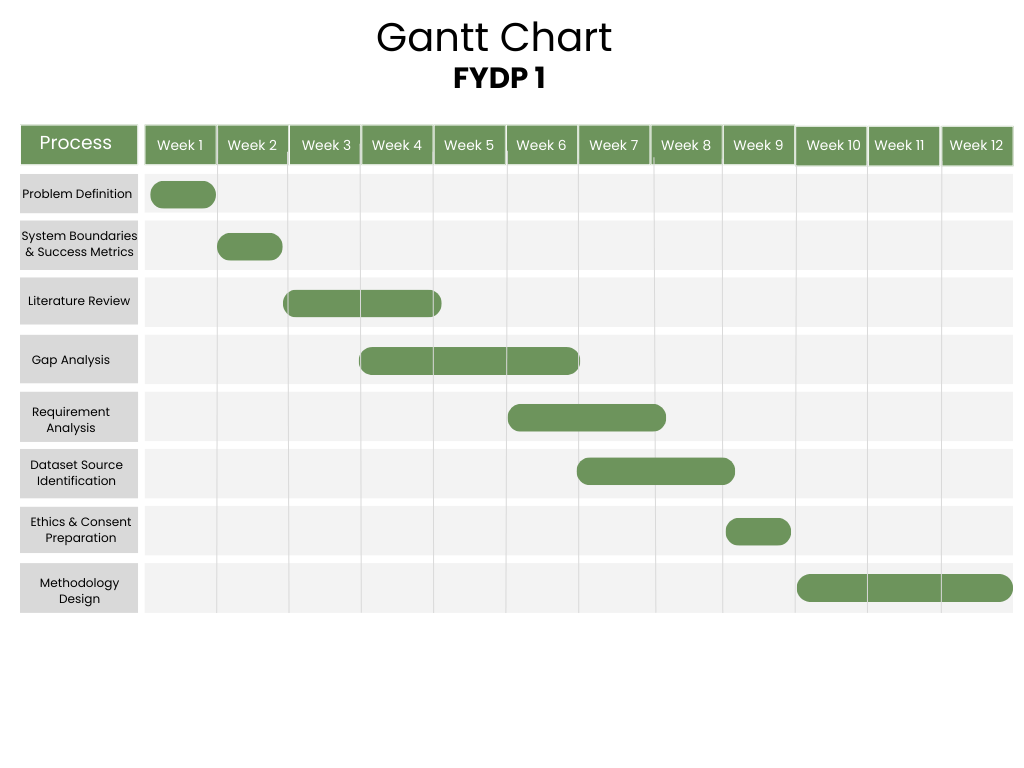
\includegraphics[width=0.8\textwidth]{Gantt Chart for FYDP - 1.png}
    \caption{Gantt Chart for FYDP - 1}
    \label{fig: Gantt Chart for FYDP - 1}
\end{figure}

\noindent
The second phase designed the architecture and built the English baseline: the voice pipeline, real-time streaming over LiveKit, and the integration of the avatar renderer. Modules were built and tested separately before being combined, and continuous testing checked real-time performance, latency and stability.\\

\begin{figure}[H]
    \centering
    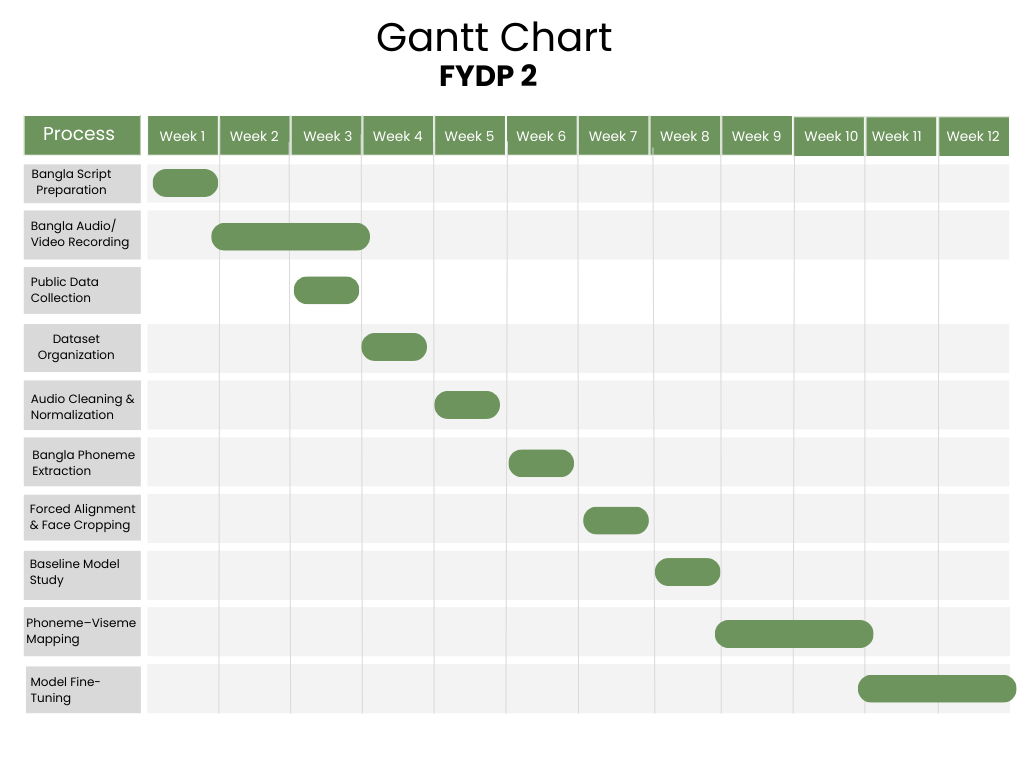
\includegraphics[width=0.8\textwidth]{Gantt Chart for FYDP - 2.png}
    \caption{Gantt Chart for FYDP - 2}
    \label{fig: Gantt Chart for FYDP - 2}
\end{figure}

\noindent
The third phase moved the system to Bangla and built Alapon: the Bangla agent, the choice of avatar model, training on Bangla video, the Bangla lip-sync expert, closing the model's performance gaps, a trial of the XLS-R encoder, the benchmark of published systems on Bangla and HDTF video, and the Bangla sound-level evaluation. The final step was the preparation of this report and the start of the journal paper.\\

\begin{figure}[H]
    \centering
    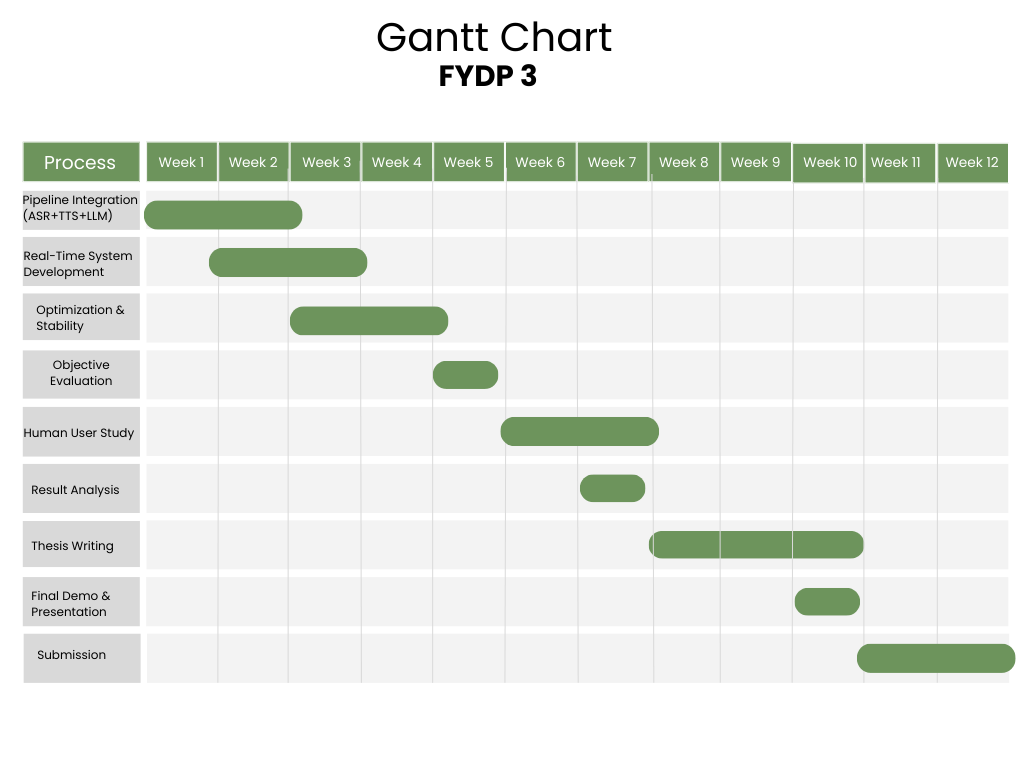
\includegraphics[width=0.8\textwidth]{Gantt Chart for FYDP - 3.png}
    \caption{Gantt Chart for FYDP - 3}
    \label{fig: Gantt Chart for FYDP - 3}
\end{figure}



\section{Task Allocation}

The work was divided among the six team members so that development of the pipeline, research and experiments, and documentation could proceed in parallel. The table below shows the distribution of roles and the main areas each member focused on.\\

\begin{table}[H]
\centering
\caption{Distribution of Project Responsibilities}
\renewcommand{\arraystretch}{1.3}
\begin{tabular}{|p{2.5cm}|p{3.5cm}|p{7.5cm}|}
\hline
\textbf{Team Member} & \textbf{Primary Role} & \textbf{Key Responsibilities \& Deliverables} \\
\hline

\textbf{Member 1} & Systems Architect + R\&D &
Integration of the conversational agent pipeline; LiveKit infrastructure; system-level latency and performance. \\
\hline

\textbf{Member 2} & R\&D and Creative &
Bangla speech and lip-sync research; comparative analysis; project imagery and posters. \\
\hline

\textbf{Member 3} & Documentation \& Lead Coordinator &
Report structure; project coordination; quality control of academic content and consistency. \\
\hline

\textbf{Member 4} & Module Developer &
Implementation of system modules; data preparation for model training; unit testing. \\
\hline

\textbf{Member 5} & Validation Engineer &
Debugging; performance monitoring; iterative refinement of system responses. \\
\hline

\textbf{Member 6} & Implementation Support &
UI/UX components; validation of software deliverables; integration testing. \\
\hline

\end{tabular}
\label{tab:project_responsibilities}
\end{table}




\section{Summary}

This chapter set out the requirements and design of the real-time Bangla conversational avatar. The requirements separate a one-off training workload, which uses cloud GPUs, from a runtime workload that must fit on a consumer laptop. The architecture connects a browser client, a Bangla speech-to-speech agent and an avatar rendering server through LiveKit and WebSockets; it was reached through a cascaded prototype and a native-audio model whose latency grew during long conversations.\\

\noindent
SyncTalk\_2D was chosen as the avatar model because it is the only candidate small and fast enough for a laptop, and the benchmark of published alternatives confirmed the choice. Building Alapon from it involved Bangla training data, a Bangla lip-sync expert, streaming audio features, closing four gaps in the model's design and training, a clean training split, and a Bangla phoneme-to-viseme mapping; a multilingual XLS-R encoder was also tried but did not work. The project plan and task allocation describe how the six-member team divided this work. Chapter~4 reports the implementation and results.\\

\chapter{Implementation and Results}

This chapter describes the implementation, how the system was tested, and the results: the effect of closing the model's gaps, Bangla sound-level results, the comparison with published systems, the leakage found in them, and speed and response time.

% ─────────────────────────────────────────────
\section{Environment Setup}
% ─────────────────────────────────────────────

The system follows the modular architecture described in Chapter~3. The project repository is organised into three main modules and one evaluation module:

\begin{itemize}
    \item \texttt{agent}: the LiveKit Agents application running the Bangla conversational agent on Gemini 3.1 Flash Live, with local voice-activity detection. An English agent is kept as a baseline.
    \item \texttt{frontend}: a Flask token server and a browser client showing the avatar video and a live transcript, with connect, disconnect and microphone-mute controls.
    \item \texttt{SyncTalk\_2D}: Alapon, the avatar model, and a FastAPI server that turns reply audio into video frames. Trained models are stored under \texttt{checkpoint/alapon/}.
    \item \texttt{benchmark}: the scoring code used for every system in Section~\ref{sec:results}, so that all systems are measured by the same code.
\end{itemize}

\noindent
Software: Python~3.10, PyTorch~2.2 (CUDA), OpenCV, FFmpeg, Librosa, FastAPI, LiveKit Agents and the Gemini API. Training and benchmarking used Google Colab GPUs. All speed measurements were made on the target laptop: AMD Ryzen 7 5800H, 8~GB RAM, NVIDIA RTX 3050 Laptop GPU (4~GB).

% ─────────────────────────────────────────────
\section{Testing and Evaluation}
\label{sec:testing}
% ─────────────────────────────────────────────

\textbf{Test data.}

\begin{itemize}
    \item \textbf{Bangla test clip:} the last 772 frames (31 seconds) of the Bangla recording. The published systems never saw this video. Alapon was trained before we found that the training data included these frames (Section~3.2, item 6), so its results on this clip for lip-sync, reconstruction and Bangla sounds may be somewhat optimistic; a clean retrain is in progress. Two tests are not affected: the silence test, because the extended mask hides the pixels the model would copy, and the six-speaker test, because its audio is new.
    \item \textbf{Six new Bangla voices:} audio from six speakers in our corpus that Alapon had never heard, used to drive the avatar's face.
    \item \textbf{HDTF \cite{zhang2021hdtf}:} a public English talking-head dataset; six speakers, one 31-second clip each, used to check the published systems on a second dataset.
\end{itemize}

\noindent
\textbf{Metrics.}

\begin{center}
\renewcommand{\arraystretch}{1.3}
\begin{tabular}{|p{3.6cm}|p{7.4cm}|p{2.4cm}|}
\hline
\textbf{Metric} & \textbf{What it measures} & \textbf{Better} \\
\hline
LSE-D & Lip-sync distance between mouth and audio & Lower \\
\hline
LSE-C & Lip-sync confidence & Close to real video \\
\hline
Mouth moving during silence & \% of frames with the mouth open when the model is driven by silent audio & Lower \\
\hline
Articulation & How often the mouth opens during speech, relative to the real speaker (1.00 = same) & Close to 1.00 \\
\hline
Open $\div$ closed & Mouth opening on \bn{আ অ} divided by mouth opening on \bn{প ফ ব ভ ম} & Close to real speaker \\
\hline
PSNR, SSIM, MAE & How closely the generated mouth region matches the real one & Higher, higher, lower \\
\hline
Speed, GPU memory & Frames per second and memory on the laptop & Higher / lower \\
\hline
\end{tabular}
\end{center}

\noindent
Lip-sync is scored with the original SyncNet \cite{chung2016outoftime}, which is independent of the model we trained. \textbf{Real video is scored too, as a reference:} a real person is perfectly in sync with their own voice, so a system should come \textit{close to} the real-video score, not above it. LSE-C reproduces to within about $\pm$0.04, so smaller differences are not meaningful.\\

\noindent
The mouth counts as open when the gap between the inner lips exceeds 3\% of the face width. This threshold sits in the middle of the real speaker's range, so the silence and articulation measures repeat to within about $\pm$2 percentage points; differences smaller than that are not meaningful.\\

\noindent
\textbf{Compared systems.} Four published methods, six checkpoints: Wav2Lip \cite{prajwal2020wav2lip} (GAN and non-GAN checkpoints), IP-LAP \cite{zhong2023iplap}, MuseTalk 1.0 and 1.5 \cite{zhang2024musetalk}, and LatentSync 1.5 \cite{li2024latentsync}. We ran all of them ourselves, on the same clips, with the same scoring code. SyncTalk\_2D before the fix, trained by us on the same Bangla data with the original mask, is included as a control.

% ─────────────────────────────────────────────
\section{Results and Discussion}
\label{sec:results}
% ─────────────────────────────────────────────

\subsection{Closing the mouth-mask gap}
\label{sec:maskfix}

\begin{table}[H]
    \centering
    \caption{SyncTalk\_2D before and after the mouth-mask change (Bangla test clip)}
    \label{tab:maskfix}
    \renewcommand{\arraystretch}{1.3}
    \begin{tabular}{lcc}
        \hline
        & \textbf{Before fix} & \textbf{Alapon} \\
        \hline
        Mouth moving during silence $\downarrow$ & 41\% & \textbf{0.1\%} \\
        LSE-C (real video: 5.14) & 5.16 & 5.11 \\
        Articulation (real video: 1.00) & 1.05 & 0.94 \\
        \hline
        \multicolumn{3}{l}{\textit{Mouth-region reconstruction: original model (19 epochs) against Alapon (59 epochs)}} \\
        \hline
        & \textbf{Original model} & \textbf{Alapon} \\
        \hline
        PSNR $\uparrow$ & 29.8 dB & \textbf{33.1 dB} \\
        SSIM $\uparrow$ & 0.88 & \textbf{0.91} \\
        MAE $\downarrow$ & 0.021 & \textbf{0.014} \\
        \hline
    \end{tabular}
\end{table}

\noindent
Before the fix, the avatar's mouth moved in 41\% of frames even when there was no sound at all. The real speaker opens their mouth in about half of all frames, so the model was reproducing about 80\% of the real mouth movement without any audio: it was copying the visible jaw instead of listening. After the fix this drops to 0.1\%. The mouth still moves normally with speech: it opens 94\% as often as the real speaker's.\\

\noindent
The LSE-C row shows why the silence test is needed: the lip-sync score is the same before and after the fix within its precision (5.16 against 5.11), so the standard metric alone could not have revealed the problem.\\

\noindent
The reconstruction rows compare the original Bangla-trained model with Alapon. They reflect all of Alapon's changes together and its longer training, not the mask alone. Covering the jaw on its own makes reconstruction slightly harder: in the experiment of Table~\ref{tab:jawrows}, training error rose from 0.0178 to 0.0202 as the jaw rows were hidden, because the model loses a shortcut.\\

\noindent
To confirm the cause of the leak, we trained six identical models that differ only in how many rows of the jaw stay visible (Table~\ref{tab:jawrows}).

\begin{table}[H]
    \centering
    \caption{Visible jaw rows against mouth movement during silence}
    \label{tab:jawrows}
    \renewcommand{\arraystretch}{1.3}
    \begin{tabular}{lcccccc}
        \hline
        \textbf{Visible jaw rows} & \textbf{10 (original)} & \textbf{8} & \textbf{6} & \textbf{4} & \textbf{2} & \textbf{0 (fixed)} \\
        \hline
        Mouth moving during silence & 39\% & 36\% & 26\% & 33\% & 36\% & \textbf{8\%} \\
        LSE-C & 5.07 & 5.09 & 4.88 & 4.98 & 5.14 & 4.93 \\
        \hline
    \end{tabular}
\end{table}

\begin{figure}[H]
    \centering
    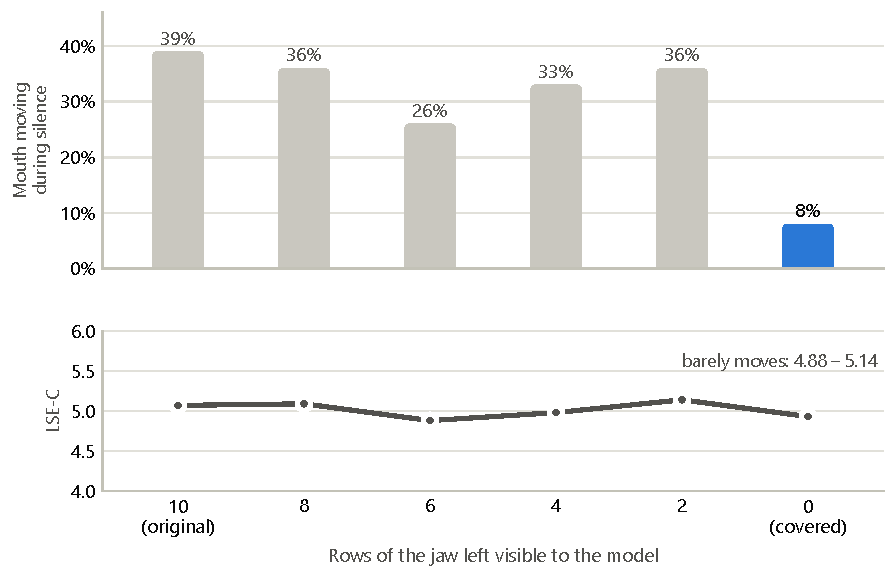
\includegraphics[width=\textwidth]{fig_jaw_rows.pdf}
    \caption{Mouth movement during silence and LSE-C against the number of visible jaw rows}
    \label{fig:jawrows}
\end{figure}

\noindent
Only covering the jaw completely stops the copying; leaving even two rows visible does not. Across all six models the LSE-C score barely changes and shows no trend. These six models were trained without the lip-sync loss; Alapon, which adds it, reaches 0.1\%.

\subsection{Bangla sound-level evaluation}
\label{sec:phoneme}

To check that the mouth follows Bangla \textit{sounds}, not just loudness, we labelled every video frame with the Bangla sound being spoken and measured how far the mouth is open for each group of sounds in Table~\ref{tab:viseme}. A Bangla speech-recognition model \cite{arijitx_bengali} marks when each written Bangla letter is spoken; the inherent vowel \bn{অ}, which is usually not written, is therefore only partly captured. Mouth opening is the gap between the inner lips divided by the width of the face.\\

\noindent
The speech-recognition model marks a sound slightly after the lips form it. For the six-speaker test (Table~\ref{tab:sixspk}) this offset was set once, on the real video (80~ms), and applied unchanged to both models. For Table~\ref{tab:phoneme}, each video was scored at the offset within $\pm$240~ms that best separates its own open and closed sounds, so that no system is penalised for a constant delay; every system except IP-LAP settled at the same 80~ms.

\begin{table}[H]
    \centering
    \caption{Mouth opening for closed and open Bangla sounds (test clip)}
    \label{tab:phoneme}
    \renewcommand{\arraystretch}{1.3}
    \begin{tabular}{lccc}
        \hline
        \textbf{System} & \textbf{Closed (\bn{প ফ ব ভ ম})} & \textbf{Open (\bn{আ অ})} & \textbf{Open $\div$ closed} \\
        \hline
        Real video & 0.011 & 0.045 & 4.0$\times$ \\
        \textbf{Alapon (ours)} & \textbf{0.011} & \textbf{0.043} & \textbf{3.8$\times$} \\
        SyncTalk\_2D, before fix & 0.015 & 0.045 & 3.0$\times$ \\
        Wav2Lip (GAN) & 0.018 & 0.053 & 3.0$\times$ \\
        Wav2Lip (non-GAN) & 0.014 & 0.041 & 3.0$\times$ \\
        LatentSync 1.5 & 0.010 & 0.031 & 3.1$\times$ \\
        MuseTalk 1.5 & 0.009 & 0.025 & 2.8$\times$ \\
        MuseTalk 1.0 & 0.005 & 0.018 & 3.5$\times$ \\
        IP-LAP & 0.016 & 0.029 & 1.9$\times$ \\
        \hline
    \end{tabular}
\end{table}

\begin{figure}[H]
    \centering
    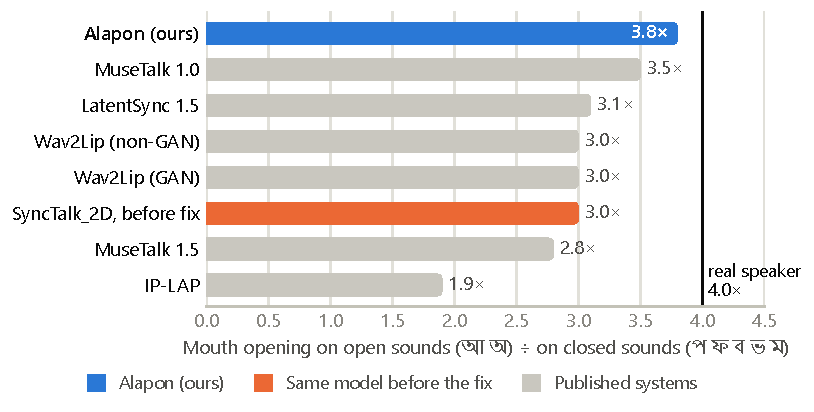
\includegraphics[width=\textwidth]{fig_bangla_sounds.pdf}
    \caption{Open $\div$ closed Bangla sounds on the test clip; the vertical line is the real speaker}
    \label{fig:banglasounds}
\end{figure}

\begin{itemize}
    \item \textbf{Alapon has the contrast closest to the real speaker} (3.8$\times$ against 4.0$\times$). Its lips close on \bn{প}, \bn{ব}, \bn{ম} as far as the real speaker's (0.011) and open on \bn{আ} almost as wide (0.043 against 0.045).
    \item \textbf{Before the fix}, the model did not close its lips fully on \bn{প}, \bn{ব}, \bn{ম} (0.015), because a lip closure does not show in the jaw it was copying. Alapon raised the contrast from 3.0$\times$ to 3.8$\times$.
    \item \textbf{Wav2Lip} opens too wide on \bn{আ} (GAN: 0.053) and does not fully close on \bn{প}, \bn{ব}, \bn{ম}. \textbf{LatentSync} closes correctly but opens too little on \bn{আ} (0.031).
    \item \textbf{MuseTalk and IP-LAP} barely move; MuseTalk 1.0's ratio looks reasonable only because both of its numbers are tiny.
\end{itemize}

\noindent
The published systems never saw this video, so the test is fair to them. Alapon's row shares the caveat in Section~\ref{sec:testing}, so we also tested it on voices it had never heard: six Bangla speakers from our corpus. In this test the face is still our speaker's, but the audio comes from someone else, so the mouth can only follow the audio.

\begin{table}[H]
    \centering
    \caption{Open $\div$ closed with six new Bangla speakers}
    \label{tab:sixspk}
    \renewcommand{\arraystretch}{1.3}
    \begin{tabular}{lcc}
        \hline
        \textbf{Speaker} & \textbf{Alapon} & \textbf{Before fix} \\
        \hline
        02 & \textbf{2.55$\times$} & 1.99$\times$ \\
        04 & \textbf{1.96$\times$} & 1.49$\times$ \\
        08 & \textbf{2.01$\times$} & 1.82$\times$ \\
        11 & \textbf{1.88$\times$} & 1.63$\times$ \\
        22 & \textbf{3.18$\times$} & 1.76$\times$ \\
        23 & \textbf{2.76$\times$} & 1.59$\times$ \\
        \hline
        \textbf{All six} & \textbf{2.3$\times$} & \textbf{1.7$\times$} \\
        \hline
    \end{tabular}
\end{table}

\begin{figure}[H]
    \centering
    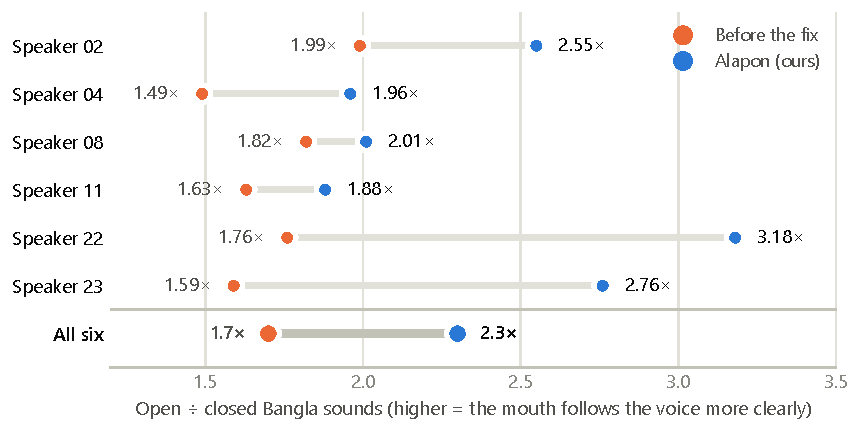
\includegraphics[width=\textwidth]{fig_six_speakers.pdf}
    \caption{Open $\div$ closed Bangla sounds for six new speakers, before the fix and with Alapon}
    \label{fig:sixspeakers}
\end{figure}

\noindent
Alapon keeps a clear contrast between open and closed sounds with new voices, and is higher than the model before the fix for \textbf{every one of the six speakers}. The model before the fix copies the mouth of the original video, which is saying different words, so its mouth separates the sounds less. The contrast is smaller than the real speaker's (4.0$\times$), so Alapon follows new voices less strongly than the voice it was trained on.\\

\noindent
We also measured lip width to separate rounded sounds (\bn{উ}, \bn{ও}) from spread ones (\bn{ই}, \bn{এ}), but it did not show a clear difference between the systems, so we do not claim that the mouth \textit{shape} matches each sound.

\subsection{Comparison with published systems}
\label{sec:comparison}

\begin{table}[H]
    \centering
    \caption{Comparison on the Bangla test clip}
    \label{tab:comparison_bn}
    \renewcommand{\arraystretch}{1.3}
    \begin{tabular}{lrcccc}
        \hline
        \textbf{System} & \textbf{Checkpoint} & \textbf{LSE-D $\downarrow$} & \textbf{LSE-C} & \textbf{Silence $\downarrow$} & \textbf{Articulation} \\
        \hline
        Real video & -- & 7.39 & 5.14 & -- & 1.00 \\
        \textbf{Alapon (ours)} & \textbf{49 MB} & 7.30 & 5.11 & \textbf{0.1\%} & 0.94 \\
        SyncTalk\_2D, before fix & 49 MB & 7.32 & 5.16 & 41\% & 1.05 \\
        Wav2Lip (GAN) & 436 MB$^{\dagger}$ & 7.26 & 6.08 & 46\% & 1.21 \\
        Wav2Lip (non-GAN) & 436 MB$^{\dagger}$ & 6.83 & 6.44 & 0.8\% & 1.05 \\
        LatentSync 1.5 & 5,072 MB & 7.29 & 5.09 & 36\% & 0.79 \\
        MuseTalk 1.5 & 3,400 MB & 7.86 & 4.90 & 0.4\% & 0.53 \\
        MuseTalk 1.0 & 3,400 MB & 7.72 & 4.67 & 0.1\% & 0.22 \\
        IP-LAP & 475 MB & 8.71 & 4.36 & 20\% & 0.76 \\
        \hline
    \end{tabular}

    \vspace{0.3em}
    {\footnotesize Silence: mouth moving during silence. Real video is not a model, so it has no checkpoint and cannot be driven by silent audio. $^{\dagger}$Includes training optimiser state.}
\end{table}

\begin{figure}[H]
    \centering
    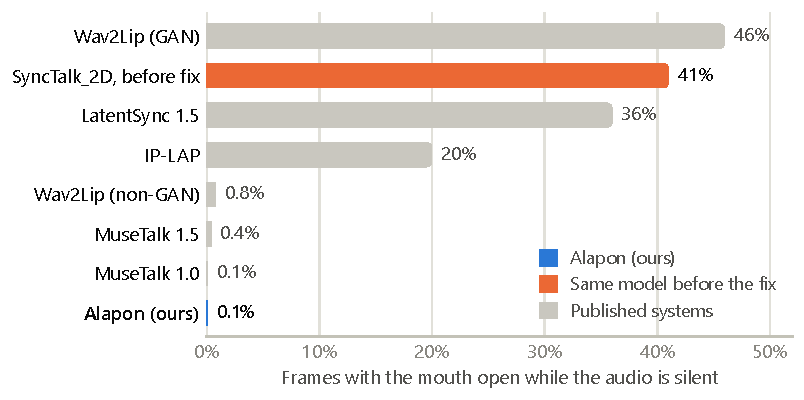
\includegraphics[width=\textwidth]{fig_silence_bangla.pdf}
    \caption{Mouth movement during silence on the Bangla test clip}
    \label{fig:silence}
\end{figure}

\begin{itemize}
    \item \textbf{Alapon matches real video on lip-sync} (5.11 against 5.14), as does LatentSync (5.09); both differences are within the scorer's precision. LatentSync's checkpoint, however, is about 100 times larger than Alapon's, and its mouth moves during silence in 36\% of frames.
    \item \textbf{Both Wav2Lip checkpoints score above real video} (6.08 and 6.44 against 5.14). This is not better lip-sync: Wav2Lip was trained against the same SyncNet that scores it.
    \item \textbf{Four systems stay below 1\% during silence}: Alapon, both MuseTalk versions and Wav2Lip (non-GAN); they are equal within the measure's precision. But MuseTalk also barely moves during speech (articulation 0.53 and 0.22): it avoids mistakes by barely moving at all. Alapon is still in silence and moves almost as much as the real speaker in speech (0.94).
\end{itemize}

\subsection{Leakage in published systems}
\label{sec:leakage}

Having found that SyncTalk\_2D copied the mouth from its input video, we asked whether the published systems do the same. We drove all six published checkpoints with silent audio on the Bangla clip and on six HDTF speakers, and scored them with the same code as Alapon.

\begin{table}[H]
    \centering
    \caption{Published systems on the public English dataset HDTF (six speakers, averages)}
    \label{tab:hdtf}
    \renewcommand{\arraystretch}{1.3}
    \begin{tabular}{lccccc}
        \hline
        \textbf{System} & \textbf{LSE-D $\downarrow$} & \textbf{LSE-C} & \textbf{Above real?} & \textbf{Silence $\downarrow$} & \textbf{Articulation} \\
        \hline
        Real video & 7.42 & 8.01 & -- & -- & 1.00 \\
        Wav2Lip (GAN) & 6.93 & 8.75 & \textbf{yes} & 24\% & 1.03 \\
        Wav2Lip (non-GAN) & 6.69 & 8.94 & \textbf{yes} & 8\% & 0.98 \\
        LatentSync 1.5 & 6.70 & 8.82 & \textbf{yes} & 24\% & 0.64 \\
        MuseTalk 1.5 & 7.12 & 8.38 & \textbf{yes} & 46\% & 0.99 \\
        MuseTalk 1.0 & 7.72 & 7.52 & no & 41\% & 0.75 \\
        IP-LAP & 7.07 & 7.88 & no & 10\% & 0.34 \\
        \hline
    \end{tabular}
\end{table}

\begin{figure}[H]
    \centering
    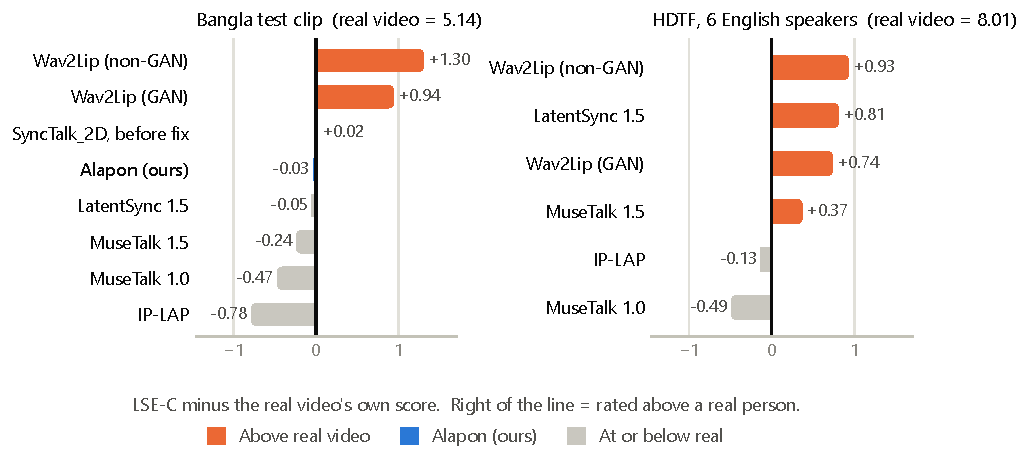
\includegraphics[width=\textwidth]{fig_lsec_vs_real.pdf}
    \caption{LSE-C of each system minus the real video's own score, on both datasets}
    \label{fig:lsecreal}
\end{figure}

\begin{figure}[H]
    \centering
    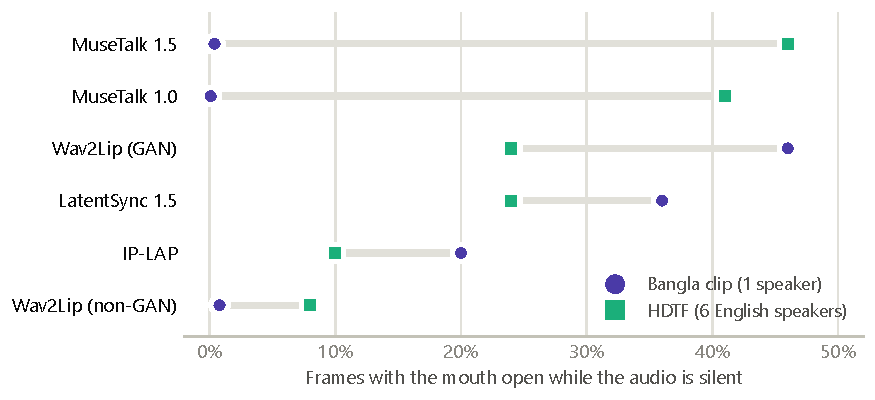
\includegraphics[width=\textwidth]{fig_leak_two_datasets.pdf}
    \caption{Mouth movement during silence for the same systems on the Bangla clip and on HDTF}
    \label{fig:twodatasets}
\end{figure}

\noindent
Alapon is not in this table: it is person-specific and would have to be trained separately for each HDTF speaker. Five findings follow from Tables~\ref{tab:maskfix}, \ref{tab:jawrows}, \ref{tab:comparison_bn} and \ref{tab:hdtf}.

\begin{enumerate}
    \item \textbf{Five of the six published checkpoints leak on at least one dataset.} Their mouths moved during silence in 20--46\% of frames on at least one of the two datasets. Only Wav2Lip (non-GAN) stayed low on both (0.8\% on Bangla, 8\% on HDTF, the level of our own jaw-covered models in Table~\ref{tab:jawrows}). The gap we closed in SyncTalk\_2D is not unique to it.
    \item \textbf{The standard lip-sync metric scores generated video above real video.} On HDTF, four of six systems score above the real speakers on LSE-C. For Wav2Lip and Wav2Lip GAN the difference is statistically significant across the six speakers even after correcting for testing six systems (paired t-test, p = 0.004 and 0.007); LatentSync's (p = 0.02) is not, after correction. Real video is the ceiling by definition, so a metric that ranks synthesis above it is not measuring what its name claims.
    \item \textbf{The lip-sync metric cannot see leakage.} In Table~\ref{tab:jawrows}, covering the jaw cut leakage from 39\% to 8\% while LSE-C stayed flat. We had expected the metric to \textit{reward} leakage; the experiment did not support that, and we report the negative result. What it does show is that the metric is blind to leakage: the most-leaking system on HDTF, MuseTalk 1.5, still scores above real video.
    \item \textbf{Measured leakage depends on the speaker.} A system can only copy the mouth movement that is in its input video, so speakers who move their mouths more reveal more leakage. Across the 36 speaker--system pairs on HDTF, leakage rises with the speaker's own mouth movement (rank correlation +0.64). One HDTF speaker barely opens their mouth, and nearly every system scores close to zero leakage on that speaker. We therefore propose dividing leakage by how much the real speaker moves, so that results can be compared across speakers and datasets.
    \item \textbf{One clip is not enough to judge a system.} MuseTalk 1.5 moved its mouth during silence in 0.4\% of frames on the Bangla clip but 46\% on HDTF, while LatentSync and Wav2Lip GAN leaked more on the Bangla clip than on HDTF. Leakage should be measured over several speakers and reported with its spread, including our own 0.1\%, which comes from one Bangla clip. For Alapon the extended mask itself is the stronger evidence: the model cannot copy jaw pixels it can no longer see.
\end{enumerate}

\noindent
These findings go beyond the FYDP system and are the subject of the journal paper described in Section~\ref{sec:journal}.

\subsection{Speed and response time}
\label{sec:speed}

\begin{table}[H]
    \centering
    \caption{Performance on the laptop (RTX 3050, 4 GB)}
    \label{tab:performance}
    \renewcommand{\arraystretch}{1.3}
    \begin{tabular}{p{5.6cm}cc}
        \hline
        & \textbf{Result} & \textbf{Requirement} \\
        \hline
        Model size & 49 MB & -- \\
        Rendering speed & 30 frames per second (33 ms per frame) & 25 fps \\
        GPU memory used & 0.3 GB of 4 GB & -- \\
        Response time (user stops speaking $\rightarrow$ avatar answers) & 1.5--2 s & 1--2 s \\
        \hline
    \end{tabular}
\end{table}

\noindent
The avatar renders faster than the 25 frames per second it needs, using less than a tenth of the laptop's GPU memory. The response time was measured in live sessions from the agent's timing log. Part of it is deliberate: the system waits for 0.55 seconds of silence before answering, so that natural Bangla pauses are not cut off. Gemini's reply time stays flat across a long conversation.

\subsection{Bangla audio encoder (XLS-R)}
\label{sec:xlsr}

We also trained the model with a multilingual speech encoder, XLS-R \cite{babu2022xlsr}, in place of the default audio features, expecting it to represent Bangla sounds better. It did not work. The first attempt used the encoder's last layer, whose output barely changes from frame to frame, so the lip-sync expert could not learn at all. With a middle layer (layer 12) it learned, but weakly: it separated in-sync from out-of-sync audio about half as well as the expert trained on the default features. The avatar trained against this weaker expert moved its mouth more during silence than the default model, so Alapon uses the default audio features. The default features come from an encoder pre-trained specifically for audio--visual synchronisation, which is a strong starting point; a general speech representation would need more than five minutes of a single speaker to learn the mapping to mouth movement.

\subsection*{Discussion}

\begin{enumerate}
    \item \textbf{Closing the jaw gap was the key result.} It stopped the model copying mouth movement from the video (41\% $\rightarrow$ 0.1\%) and sharpened Bangla sounds (open $\div$ closed 3.0$\times$ $\rightarrow$ 3.8$\times$).
    \item \textbf{Alapon follows Bangla sounds.} Its lips close on \bn{প}/\bn{ব}/\bn{ম} and open on \bn{আ} closer to the real speaker than any other system, and still clearly for six Bangla speakers it had never heard (2.3$\times$ against 1.7$\times$ before the fix).
    \item \textbf{Small and fast.} At 49~MB, Alapon reaches the real-video lip-sync score, as a 5~GB model does, and renders at 30~fps on a laptop.
    \item \textbf{The leak is a field-wide problem.} Five of the six published systems we tested leak on at least one dataset, and the standard lip-sync metric neither detects leakage nor keeps generated video below real video. Evaluating a talking head needs the silence test and the real-video reference alongside the lip-sync score.
    \item \textbf{Meets the requirements.} 30~fps against the 25~fps target, and a 1.5--2~s response against the 1--2~s target.
\end{enumerate}

% ─────────────────────────────────────────────
\section{Summary}
% ─────────────────────────────────────────────

Alapon, the avatar model, is 49~MB, renders at 30 frames per second on a laptop RTX 3050 using 0.3~GB of GPU memory, and the system answers within 1.5--2 seconds. Covering the jaw reduced mouth movement during silence from 41\% to 0.1\% and raised the contrast between open and closed Bangla sounds from 3.0$\times$ to 3.8$\times$, against 4.0$\times$ for the real speaker. For six Bangla speakers it had never heard, its mouth opens 2.3 times wider on \bn{আ} than on \bn{প}/\bn{ব}/\bn{ম}, against 1.7 times before the fix. On the Bangla test clip its lip-sync score matches real video (5.11 against 5.14). The same silence test showed that five of the six published systems leak on at least one dataset, and that the standard lip-sync metric scores generated video above real video. The multilingual XLS-R encoder did not work and was not used in Alapon.

\chapter{Standards and Design Constraints}

This chapter relates the project to professional and ethical standards, describes the constraints that shaped its design, analyses its cost, and shows that it constitutes a complex engineering problem.

\section{Compliance with the Standards}
The system aligns with established professional and ethical standards, including the ACM Code of Ethics and Professional Conduct, the ASME Code of Ethics and the IEEE Code of Ethics. The following sections set out the specific principles that apply.

\subsection{Software Standards}
The following software standards are in line with the scope of the system.\\


\textbf{ACM Code of Ethics and Professional Conduct -- Principle 2.1: Strive to achieve high quality in both the processes and products of professional work}

\noindent
The system uses established models, careful adaptation and systematic testing, and every result reported is measured with a documented, repeatable procedure.

\vspace{0.5cm}


\textbf{ACM Code of Ethics -- Principle 2.5: Give comprehensive and thorough evaluations of computer systems and their impacts, including possible risks}

\noindent
The system is evaluated on lip-sync accuracy, mouth movement during silence, reconstruction quality, Bangla sounds, speed and response time, against six published checkpoints on two datasets, and its limitations are reported explicitly (Section~\ref{sec:limitation}).

\vspace{0.5cm}


\textbf{ACM Code of Ethics -- Principle 2.7: Foster public awareness and understanding of computing, related technologies, and their consequences}

\noindent
By documenting how the avatar works, what it can and cannot do, and how talking-head metrics can mislead, the project promotes understanding of these technologies and their impacts.

\vspace{0.5cm}


\textbf{ACM Code of Professional Responsibilities -- Code 2.2: Maintain high standards of professional competence, conduct, and ethical practice}

\noindent
The team followed ethical practice throughout the project.

\vspace{0.5cm}


\textbf{ACM Code of Professional Responsibilities -- Code 2.9: Design and implement systems that are robustly and usably secure}

\noindent
Access to the system is controlled by session tokens, and the design aims to prevent misuse of the avatar and to remain intuitive and safe to operate.

\vspace{0.5cm}


\textbf{IEEE Code of Ethics -- Clause 3: Be honest and realistic in stating claims or estimates based on available data}

\noindent
Every performance figure in this report is measured, and its source is recorded. Where an earlier estimate was not supported by measurement, such as the end-to-end latency figure of the FYDP-1 design, it has been replaced with measured values. Where a result has a known weakness, such as the training data that overlapped the test frames, or an expectation that the experiments did not support, that is stated.

\vspace{0.5cm}


\textbf{IEEE Code of Ethics -- Clause 6: Maintaining technical competence in software and hardware}

\noindent
The solution lies within the team's field of study, Computer Science and Engineering.

\vspace{0.5cm}


\textbf{Fundamental Canons of ASME Code 2: Engineers shall perform services only in the areas of their competence}

\noindent
The project draws on machine learning, deep learning, computer vision and real-time systems, all within the team's discipline of Computer Science and Engineering.



\subsection{Hardware Standards}

The following hardware standards are in line with the scope of the system.\\


\textbf{ASME Code of Ethics -- Fundamental Canon 2: Engineers shall perform services only in areas of their competence}

\noindent
The project uses consumer GPUs and cloud GPU resources that match the team's expertise in machine learning and neural rendering.

\vspace{0.5cm}


\textbf{ASME Code of Ethics -- Fundamental Canon 1: Engineers shall hold paramount the safety, health, and welfare of the public}

\noindent
Training runs on cloud GPUs and the system runs on an ordinary laptop, so it poses no particular physical risk. The project is not intended for safety-critical use without further validation.

\vspace{0.5cm}


\textbf{IEEE Code of Ethics -- Clause 1: Hold paramount the safety, health, and welfare of the public}

\noindent
The hardware used is standard consumer and cloud computing equipment and poses no direct physical risk to the public.

\vspace{0.5cm}


\textbf{IEEE Code of Ethics -- Clause 6: Maintain and improve technical competence}

\noindent
Hardware choices are documented and measured, for example the choice of a laptop-class GPU as the runtime target, and the team worked within its technical training.


\subsection{Communication Standards}

The following communication standards are in line with the scope of the system.\\


\textbf{ACM Code of Ethics -- Principle 1.3: Be honest and trustworthy}

\noindent
The methodology, dataset limitations and model assumptions are documented in this report and in the project's code, including results that did not support our initial expectations (Sections~\ref{sec:leakage} and~\ref{sec:xlsr}).

\vspace{0.5cm}


\textbf{ACM Code of Ethics -- Principle 2.3: Know and respect existing rules pertaining to professional work}

\noindent
The project follows applicable rules on data handling, privacy and intellectual property. The Bangla corpus is used for research only and is not redistributed until the licences of its source recordings have been traced.

\vspace{0.5cm}


\textbf{IEEE Code of Ethics -- Clause 5: Improve the understanding of technology, its appropriate application, and potential consequences}

\noindent
The project provides documentation and demonstration videos explaining how the system works, its intended uses and its limitations, particularly for a low-resource language. The performance gaps found in SyncTalk\_2D and the weaknesses found in the standard evaluation are being reported to the research community through the journal paper.


\subsection{Societal Standards}

The following societal standards are in line with the scope of the system.\\


\textbf{ACM Code of Ethics -- Principle 1.1: Contribute to society and to human well-being}

\noindent
The system serves Bangla speakers, who are underserved by current AI technology, and is designed to be deployable where resources are limited.

\vspace{0.5cm}


\textbf{ACM Code of Ethics -- Principle 1.6: Respect privacy}

\noindent
The avatar is trained on video of a speaker who consented to its use \todo{confirm: the \texttt{redwan} recording is of team member Sheikh Redwanul Islam, recorded with his consent}. The system performs no identity recognition or surveillance. The user's speech is sent to the Gemini API to generate replies, which users should be told.

\vspace{0.5cm}


\textbf{IEEE Code of Ethics -- Clause 10: Assist colleagues and co-workers in their professional development}

\noindent
The project's source code and evaluation tools are documented so that others can reproduce and build on the work. The Bangla corpus will be released once the licences of its source recordings have been traced.




\section{Design Constraints}

The design of the Real-Time Bangla Speech-Driven Avatar Generation system was shaped by several practical and contextual constraints. The subsections below explain the key constraints.\\

\subsection{Economic Constraint}
High-fidelity talking-head models usually need large GPUs, large datasets and cloud servers, which small institutions cannot afford. The system addresses this directly: its avatar model, Alapon, is 49~MB, renders in real time on a consumer laptop GPU using 0.3~GB of memory, and needs no cloud GPU at runtime. Training uses modest cloud GPU time once per avatar. All tools and libraries are free or open-source, and the training data is locally collected Bangla video.

\subsection{Ethical Constraint}
A system that generates realistic facial movement from speech carries risks of impersonation, deepfakes and privacy violation. To limit these, the avatar is trained only on footage of a speaker who consented, the system is intended for controlled and transparent use, and it is not used to produce false or unauthorised representations of real people. The Bangla corpus was assembled from publicly available recordings for research; the speakers did not individually consent, so the corpus is not redistributed, and its release depends on tracing the source licences. Informed consent, anonymisation where necessary, and responsible data processing guide any further data collection, including the planned human evaluation.


\subsection{Social Constraint}

Language inclusivity and cultural representation are central. Current talking-head systems focus on English, which disadvantages speakers of low-resource languages such as Bangla. This system is built specifically for Bangla users, with attention to Bangla phonetics, formal register and speech rhythm.\\

\noindent
Bangla also varies by dialect in pronunciation, intonation and vocabulary, which makes a single model representative of all speakers difficult to build from limited data. The corpus includes 24 speakers, but it has not yet been audited for balance across gender, region or speaking style.


\section{Cost Analysis}
The project was planned to be cost-effective and feasible in an academic setting. Because it is almost entirely software-based, its financial requirements are low.

The main considerations of cost in the project are as follows:

\begin{itemize}
    \item \textbf{Hardware Resources:}\\
    The system runs on a personal laptop. The avatar needs a CUDA-capable GPU, but a consumer laptop GPU is sufficient; no specialised hardware is required.

    \item \textbf{Software Resources:}\\
    All development tools, programming languages, deep learning frameworks and audio--visual libraries are free or open-source, so there are no licensing costs.

    \item \textbf{Data and Experimentation:}\\
    Training and evaluation use locally collected Bangla video and a public benchmark (HDTF), so no paid datasets are needed.

    \item \textbf{Operational Costs:}\\
    The avatar runs locally. The conversational model is accessed through the Gemini API.
\end{itemize}

\begin{table}[h]
\centering
\caption{Detailed Cost}
\small
\begin{tabularx}{\textwidth}{|l|l|X|l|l|}
\hline
\textbf{Environment} & \textbf{Component} & \textbf{Used Component} & \textbf{Price} & \textbf{Training} \\ \hline

\multirow{3}{*}{Local}
& CPU & AMD Ryzen 7 5800H & Owned & \multirow{3}{*}{N/A} \\ \cline{2-4}
& GPU & RTX 3050 Laptop, 4 GB & Owned &  \\ \cline{2-4}
& RAM & 8 GB RAM & Owned &  \\ \hline

\multirow{4}{*}{Cloud}
& Google Colab Pro & A100, L4, T4 & \todo{spend} & \multirow{4}{*}{\todo{hours}} \\ \cline{2-4}
& Kaggle & T4 & Free &  \\ \cline{2-4}
& Storage & Google Drive & Free &  \\ \cline{2-4}
& Conversational model & Google Gemini API & \todo{cost} &  \\ \hline

\end{tabularx}
\end{table}


\noindent
The cost analysis confirms that the project can be completed with very little expenditure, which makes it appropriate and sustainable for an undergraduate final year design project.






\section{Complex Engineering Problem}
\subsection{Complex Problem Solving}

Whether a problem is a complex engineering problem is determined by checking whether it satisfies the attributes P1 to P7.\\

\noindent
\textbf{P1: Depth of Knowledge Required}

\noindent
P1 is satisfied when the project requires one or more of the knowledge profiles K3, K4, K5, K6 or K8. The profiles that apply to this project are evaluated below.

\noindent
\textbf{K1: Engineering Fundamentals}
\noindent
The project uses mathematics, signal processing and computer science: audio is represented and transformed mathematically, and engineering principles govern real-time synchronisation and control.

\noindent
\textbf{K2: Discipline-Specific Knowledge}
\noindent
Core computer science applies: machine learning, computer vision, data structures, algorithms and software architecture, with frame-based video rendering and audio processing as key discipline-specific elements.

\noindent
\textbf{K3: Specialist Knowledge}
\noindent
Audio-to-visual speech synthesis requires specialist knowledge of deep learning. Lip synchronisation, phoneme-to-viseme mapping, facial landmark modelling and low-resource Bangla data make the problem highly specialised.

\noindent
\textbf{K4: Design and Development}
\noindent
The project required systematic engineering design: end-to-end pipeline modelling, system architecture design and iterative development, with trade-offs between realism, latency and computation.

\noindent
\textbf{K5: Engineering Tools, Software \& Techniques}
\noindent
Modern tools were used (Python, PyTorch, computer vision and audio processing libraries), together with optimisation techniques to achieve real-time execution.

\noindent
\textbf{K6: Impact of Engineering on Society \& Environment}
\noindent
The project considers the ethical and social consequences of deepfakes, identity, privacy and responsible AI.

\noindent
\textbf{K7: Management, Finance \& Project Management}
\noindent
Planning, scheduling, version control and time management were used throughout, within limited resources.

\noindent
\textbf{K8: Lifelong Learning:}
\noindent
The field changes rapidly; new techniques, tools and research were studied and integrated during development.

\vspace{1em}

\noindent
P1 is satisfied, as K3, K4, K5, K6, K7 and K8 all apply.\\

\noindent
\textbf{P2: Range of Conflicting Requirements}
\noindent
The project involved many conflicting requirements. A smaller model renders faster but risks poorer lip-sync; a larger one looks better but cannot run on a laptop. A longer end-of-turn wait avoids cutting the user off but makes the system feel slower. Emitting video frames earlier reduces latency but risks lip frames ahead of their audio. Identity preservation competes with generalisation to new speakers. These were balanced through measurement and testing. P2 is satisfied.

\vspace{0.7em}

\noindent
\textbf{P3: Depth of Analysis Required}
\noindent
The problem has no simple answer. Many methods exist for audio-driven lip synchronisation (viseme-based, convolutional, transformer and diffusion models), but none targets real-time Bangla lip-sync on limited hardware. The solution required a comparative benchmark of published systems, adaptation of the selected model, a causal diagnosis of why its mouth moved without audio, and an analysis of why the standard metric could not detect it. P3 is satisfied.


\vspace{0.7em}

\noindent
\textbf{P4: Familiarity of Issues}
\noindent
Real-time Bangla lip synchronisation raises issues not covered in standard coursework: audio--visual synchronisation under real-time constraints, streaming audio features that must match offline extraction, Bangla phoneme-to-viseme mapping, low-resource language data, identity-preserving generation, and the reliability of evaluation metrics. P4 is satisfied.

\vspace{0.7em}

\noindent
\textbf{P5: Extent of Applicable Codes}
\noindent
The project must follow professional and ethical codes (the ACM and IEEE Codes of Ethics and responsible-AI principles), with attention to data privacy, consent for facial data, and responsible use of AI-generated media. P5 is satisfied.

\vspace{0.7em}

\noindent
\textbf{P6: Extent of Stakeholder Involvement}
\noindent
Stakeholders include end users, educators and other deploying institutions, developers, researchers and the wider public, with differing needs for visual realism, real-time performance, ethical use and reliability. P6 is satisfied.

\vspace{0.7em}

\noindent
\textbf{P7: Interdependence}
\noindent
The audio processing, lip-motion model, rendering server, conversational agent and real-time media layer are tightly interdependent and must stay synchronised; latency, inference speed and ethical constraints follow directly from the core problem. P7 is satisfied.


\begin{center}
    \begin{table}[ht]
        \centering
        \caption{Mapping with complex problem solving.}
        \begin{tabular}{|p{0.12\textwidth}|p{0.12\textwidth}|p{0.12\textwidth}|p{0.12\textwidth}|p{0.12\textwidth}|p{0.12\textwidth}|p{0.12\textwidth}|}
        \hline
        P1& P2& P3& P4& P5& P6& P7\\
        Depth of Knowledge & Range of Conflicting Requirements & Depth of Analysis & Familiarity of Issues & Extent of Applicable Codes & Extent of Stakeholder Involvement & Inter-dependence\\
        \hline
        $\sqrt{}$ & $\sqrt{}$ & $\sqrt{}$ & $\sqrt{}$ & $\sqrt{}$ & $\sqrt{}$ & $\sqrt{}$\\
        &&&&&&\\
        \hline
        \end{tabular}
        \label{tab:p_solve}
    \end{table}
\end{center}


\subsection{Engineering Activities}

The engineering activities A1 to A5 were addressed through systematic analysis, design, implementation and evaluation, as outlined below.\\

\noindent
\textbf{A1: Range of Resources}

\noindent
The solution combines many resources: speech input, audio processing, a deep-learning lip-sync model, a rendering server, a conversational model and a real-time media layer, all of which must be coordinated to produce synchronised audio and video. Responsible data use, privacy and deployment constraints are also in scope. A1 is satisfied.

\vspace{0.5em}

\noindent
\textbf{A2: Innovation}

\noindent
The project applies audio-driven facial animation to Bangla speech, which had not been done in the open systems we reviewed. It identifies and closes four performance gaps in a publicly available model, one of which made it copy mouth shape instead of listening; introduces a Bangla sound-level evaluation; and shows, with a silent-audio test and a real-video reference, that published systems leak and that the standard metric cannot detect it. A2 is satisfied.


\vspace{0.5em}

\noindent
\textbf{A3: Level of Interaction}

\noindent
Speech processing, deep-learning inference, rendering and synchronisation interact closely, and balancing computation, visual quality and responsiveness required continual adjustment across all of them. A3 is satisfied.

\vspace{0.5em}

\noindent
\textbf{A4: Consequences for Society and Environment}

\noindent
Realistic talking avatars can improve education, communication and access to services, but also raise concerns about misuse and misinformation, which the project addresses through consent, controlled use and transparency. Because the system runs on existing consumer hardware, it avoids new hardware and limits its environmental impact. A4 is satisfied.

\vspace{0.5em}

\noindent
\textbf{A5: Familiarity}

\noindent
The problem requires knowledge beyond standard coursework: deep-learning speech-driven synthesis, real-time streaming systems and evaluation methodology. A5 is satisfied.

\vspace{0.8em}

\noindent
\textbf{Conclusion}

\noindent
These activities show a structured and systematic approach to a complex engineering problem, combining advanced AI techniques, real-time system design, iterative optimisation and ethical awareness.




\begin{center}
    \begin{table}[ht]
        \centering
                \caption{Mapping with complex engineering activities.}

        \begin{tabular}{|p{0.18\textwidth}|p{0.18\textwidth}|p{0.18\textwidth}|p{0.18\textwidth}|p{0.18\textwidth}|}
        \hline
        A1& A2& A3& A4& A5\\
        Range of resources & Innovation & Level of Interaction & Consequences for society and environment & Familiarity\\
        \hline
        $\sqrt{}$ & $\sqrt{}$ & $\sqrt{}$ & $\sqrt{}$ & $\sqrt{}$\\
        &&&&\\
        \hline
        \end{tabular}
        \label{tab:e_act}
    \end{table}
\end{center}


\section{Summary}

This chapter related the Real-Time Bangla Speech-Driven Avatar Generation system to the relevant software, hardware, communication and societal standards, and examined the economic, ethical and social constraints that shaped its design.\\

\noindent
The cost analysis shows that the project can be delivered with very little expenditure. Finally, the project was shown to be a complex engineering problem, because it integrates real-time AI processing, low-resource language adaptation, neural rendering on consumer hardware, and the evaluation of the models it depends on.

\chapter{Conclusion}

This chapter summarises the project, states its limitations, and describes the journal paper in progress and future work.

\section{Summary}

This project set out to close a gap: there was no open, real-time conversational avatar that speaks Bangla and runs on a laptop. It delivers one. A user speaks Bangla in a web browser, a speech-to-speech agent replies in formal Bangla, and a 2D avatar speaks the reply with synchronised lip movement.\\

\noindent
We chose SyncTalk\_2D, the only candidate small and fast enough for a laptop, and confirmed the choice by testing published lip-sync systems on Bangla video. We adapted it to Bangla with Bangla training video, a Bangla-trained lip-sync expert and streaming audio features. We then found four gaps in the model that limited its performance. The most important was the mouth mask: the model copied the visible jaw instead of listening, and its mouth moved in 41\% of frames during silence. Our improved model, \textbf{Alapon}, moves in 0.1\% and separates open and closed Bangla sounds almost as well as the real speaker.\\

\noindent
We then checked whether published systems have the same problem. Five of the six we tested leak on at least one dataset, and the standard lip-sync metric cannot see it; it even scores generated video above real video. These findings are being prepared as a journal paper.\\

\noindent
The completed system runs Alapon: 49~MB, 30 frames per second on a laptop RTX 3050 using 0.3~GB of GPU memory, and a reply within 1.5--2 seconds. On the Bangla test clip its lip-sync score matches real video (5.11 against 5.14).

\begin{table}[H]
\centering
\caption{Proposed against delivered}
\label{tab:delivered}
\renewcommand{\arraystretch}{1.3}
\begin{tabular}{|p{5.2cm}|p{8.3cm}|}
\hline
\textbf{Proposed in FYDP-1} & \textbf{Result} \\
\hline
Real-time Bangla conversational avatar & \textbf{Done.} Working end-to-end system running Alapon; answers in 1.5--2 s. \\
\hline
Separate speech recognition, LLM and speech synthesis & \textbf{Changed} to one speech-to-speech model (Gemini 3.1 Flash Live), which is faster. \\
\hline
Real-time on local hardware & \textbf{Done.} 30 fps on a laptop RTX 3050, 0.3 GB GPU memory. \\
\hline
End-to-end latency of 200--300 ms (FYDP-1 estimate) & \textbf{Not met.} Measured response is 1.5--2 s, including a deliberate 0.55 s wait so that Bangla pauses are not cut off; the requirement is now 1--2 s. \\
\hline
Bangla-trained SyncNet & \textbf{Done.} Retrained with mismatched pairs on the Bangla speaker and used during training. \\
\hline
Multilingual audio encoder (XLS-R) & \textbf{Tried, did not work.} Its lip-sync expert learned about half as well as with the default features; not used. \\
\hline
Bangla audiovisual dataset & \textbf{Collected.} 2.78 hours from 24 speakers; six speakers used as unseen test audio, none used for training. \\
\hline
Bangla phoneme-to-viseme mapping & \textbf{Defined and used for evaluation} (Table~\ref{tab:viseme}, Section~\ref{sec:phoneme}); not yet used in training. \\
\hline
Lip-landmark loss & \textbf{Not done.} \\
\hline
\textit{Not proposed:} model selection by benchmark & \textbf{Done.} Candidates compared on size and speed (Table~\ref{tab:candidates}). \\
\hline
\textit{Not proposed:} closing the model's performance gaps & \textbf{Done.} Four gaps addressed; mouth movement during silence 41\% $\rightarrow$ 0.1\%. \\
\hline
\textit{Not proposed:} leakage study of published systems & \textbf{Done.} Six checkpoints on Bangla and HDTF; journal paper in preparation. \\
\hline
\end{tabular}
\end{table}

\section{Limitation}
\label{sec:limitation}

\begin{itemize}
    \item \textbf{One speaker.} Alapon is trained and tested on one Bangla speaker. Each new face needs its own video and training.
    \item \textbf{Training overlapped the test frames.} The models in this report were trained before the training split was fixed, so Alapon's lip-sync, reconstruction and Bangla-sound results on the test clip may be somewhat optimistic. The silence test and the six-speaker test are not affected. A retrain on the training frames only is in progress.
    \item \textbf{Mouth opening, not mouth shape.} The lips open and close correctly for Bangla sounds, but lip width did not show that rounded and spread sounds get different shapes.
    \item \textbf{Weaker on new voices.} For new speakers the open/closed contrast is 2.3$\times$, against 4.0$\times$ for the real speaker on their own voice.
    \item \textbf{No human evaluation yet.} All results are automatic measurements; a study with native Bangla speakers is planned (Section~\ref{sec:journal}).
    \item \textbf{Cloud dependency.} The avatar runs locally, but the conversation needs the Gemini API and an internet connection.
    \item \textbf{Corpus not used for training.} The 2.78-hour corpus was used only as test audio, and its source licences must be traced before it can be released.
\end{itemize}

\section{Future Work}

\subsection{Journal Paper in Progress}
\label{sec:journal}

Following our supervisor's advice, we are turning the findings of Sections~\ref{sec:maskfix} and~\ref{sec:leakage} into a journal paper, \textbf{``Evaluation Integrity in Audio-Driven Talking-Head Generation''}. Its argument is that a widely used talking-head model was not driven by audio at all, that the field's standard evaluation ranked it as working, and that the evaluation's failure modes are specific, measurable and fixable. The target is \textit{IEEE Transactions on Multimedia}, with \textit{IEEE Transactions on Circuits and Systems for Video Technology} and \textit{Pattern Recognition} as alternatives.\\

\noindent
\textbf{Planned contributions}

\begin{enumerate}
    \item \textbf{An analysis of SyncTalk\_2D's performance gaps:} four gaps in the model's design and training, with a measured causal mechanism: a ten-pixel strip of jaw produced 91\% of all mouth motion.
    \item \textbf{Evidence that the standard lip-sync metric can rank generated video above real video}, statistically significant for two systems on a public dataset, made visible by scoring real video as a reference.
    \item \textbf{A flaw in the leakage measure and its correction.} Leakage as currently measured depends on how much the test speaker moves their mouth; dividing by the speaker's own movement makes results comparable across speakers and datasets.
    \item \textbf{A paired evaluation protocol} of leakage together with articulation that no degenerate model can pass: a frozen mouth fails articulation, a copying model fails leakage, and an over-animated mouth fails articulation.
    \item \textbf{A reproducible benchmark:} one scoring code for every system, frozen test splits, pinned environments, and a negative result reported in full.
    \item \textbf{A Bangla sound-level evaluation}, and the Bangla corpus if its source licences can be traced.
\end{enumerate}

\begin{table}[H]
\centering
\caption{Status of the journal paper}
\label{tab:journal}
\renewcommand{\arraystretch}{1.3}
\begin{tabular}{|p{8.6cm}|p{4.9cm}|}
\hline
\textbf{Work} & \textbf{Status} \\
\hline
Mask experiment with six models (Table~\ref{tab:jawrows}) & Done \\
\hline
Benchmark: six published checkpoints on Bangla and HDTF, plus Alapon and the before-fix model on Bangla, one scoring code & Done \\
\hline
Silence test for every system on both datasets & Done \\
\hline
Bangla sound-level evaluation, including six unseen speakers & Done \\
\hline
Retrain Alapon and the before-fix model on the training frames only & In progress (about 15 GPU-hours) \\
\hline
Human evaluation (below) & Planned; the critical path, 4--6 weeks \\
\hline
Further reconstruction metrics (LPIPS, FID) & Planned; about 3 days \\
\hline
Corpus licences and ethics approval & Planned \\
\hline
\end{tabular}
\end{table}

\noindent
\textbf{Human evaluation.} Native Bangla speakers will watch short (8-second) clips of Alapon, the published systems and the real speaker, in random order and without being told which is which, and rate each clip for how well the lips match the speech and how natural it looks. A 6-person pilot will check the procedure, and the main study will use at least 15 people. The ratings will then be compared with the automatic measurements, to test whether the silence test and the real-video reference agree with what people actually see better than the standard lip-sync score does. If they do not, we will not propose them.\\

\noindent
The remaining work is estimated at about six weeks, most of it the recruitment for the human evaluation.

\subsection{System Extensions}

\begin{itemize}
    \item \textbf{Bangla phoneme-level lip shape:} use the phoneme-to-viseme mapping as a training signal, so that different Bangla sounds produce visibly different mouth shapes, and narrow the gap on new voices (2.3$\times$ against 4.0$\times$).
    \item \textbf{Multi-speaker training} with the collected Bangla corpus.
    \item \textbf{A Bangla audio encoder that works:} revisit XLS-R with more training data.
    \item \textbf{Fully offline operation} with an on-device conversational model.
    \item \textbf{Pilot deployment}, starting with Bangla-medium education.
\end{itemize}



\bibliographystyle{unsrtnat}
\bibliography{fydp}
\addcontentsline{toc}{chapter}{References}

\clearpage
%\appendix

%\phantomsection

%\addcontentsline{toc}{chapter}{Appendices}
%\chapter{Amino Acids\label{appAmino}}
%\begin{figure}[h]
%\begin{center}
%\includegraphics[width=1\textwidth]{./images/background/aminoacids}
%\end{center}
%\caption{Twenty different amino acids, their structures and chemical properties.\index{Amino Acid!chemical properties}\cite{Lehninger2012}.}
%\end{figure}
%\clearpage
%\thispagestyle{empty}
%\mbox{}

%\clearpage
%\phantomsection
%\addcontentsline{toc}{chapter}{Index}
%\printindex

\end{document}
